% Options for packages loaded elsewhere
\PassOptionsToPackage{unicode}{hyperref}
\PassOptionsToPackage{hyphens}{url}
%
\documentclass[
]{book}
\usepackage{amsmath,amssymb}
\usepackage{iftex}
\ifPDFTeX
  \usepackage[T1]{fontenc}
  \usepackage[utf8]{inputenc}
  \usepackage{textcomp} % provide euro and other symbols
\else % if luatex or xetex
  \usepackage{unicode-math} % this also loads fontspec
  \defaultfontfeatures{Scale=MatchLowercase}
  \defaultfontfeatures[\rmfamily]{Ligatures=TeX,Scale=1}
\fi
\usepackage{lmodern}
\ifPDFTeX\else
  % xetex/luatex font selection
\fi
% Use upquote if available, for straight quotes in verbatim environments
\IfFileExists{upquote.sty}{\usepackage{upquote}}{}
\IfFileExists{microtype.sty}{% use microtype if available
  \usepackage[]{microtype}
  \UseMicrotypeSet[protrusion]{basicmath} % disable protrusion for tt fonts
}{}
\makeatletter
\@ifundefined{KOMAClassName}{% if non-KOMA class
  \IfFileExists{parskip.sty}{%
    \usepackage{parskip}
  }{% else
    \setlength{\parindent}{0pt}
    \setlength{\parskip}{6pt plus 2pt minus 1pt}}
}{% if KOMA class
  \KOMAoptions{parskip=half}}
\makeatother
\usepackage{xcolor}
\usepackage{color}
\usepackage{fancyvrb}
\newcommand{\VerbBar}{|}
\newcommand{\VERB}{\Verb[commandchars=\\\{\}]}
\DefineVerbatimEnvironment{Highlighting}{Verbatim}{commandchars=\\\{\}}
% Add ',fontsize=\small' for more characters per line
\usepackage{framed}
\definecolor{shadecolor}{RGB}{248,248,248}
\newenvironment{Shaded}{\begin{snugshade}}{\end{snugshade}}
\newcommand{\AlertTok}[1]{\textcolor[rgb]{0.94,0.16,0.16}{#1}}
\newcommand{\AnnotationTok}[1]{\textcolor[rgb]{0.56,0.35,0.01}{\textbf{\textit{#1}}}}
\newcommand{\AttributeTok}[1]{\textcolor[rgb]{0.13,0.29,0.53}{#1}}
\newcommand{\BaseNTok}[1]{\textcolor[rgb]{0.00,0.00,0.81}{#1}}
\newcommand{\BuiltInTok}[1]{#1}
\newcommand{\CharTok}[1]{\textcolor[rgb]{0.31,0.60,0.02}{#1}}
\newcommand{\CommentTok}[1]{\textcolor[rgb]{0.56,0.35,0.01}{\textit{#1}}}
\newcommand{\CommentVarTok}[1]{\textcolor[rgb]{0.56,0.35,0.01}{\textbf{\textit{#1}}}}
\newcommand{\ConstantTok}[1]{\textcolor[rgb]{0.56,0.35,0.01}{#1}}
\newcommand{\ControlFlowTok}[1]{\textcolor[rgb]{0.13,0.29,0.53}{\textbf{#1}}}
\newcommand{\DataTypeTok}[1]{\textcolor[rgb]{0.13,0.29,0.53}{#1}}
\newcommand{\DecValTok}[1]{\textcolor[rgb]{0.00,0.00,0.81}{#1}}
\newcommand{\DocumentationTok}[1]{\textcolor[rgb]{0.56,0.35,0.01}{\textbf{\textit{#1}}}}
\newcommand{\ErrorTok}[1]{\textcolor[rgb]{0.64,0.00,0.00}{\textbf{#1}}}
\newcommand{\ExtensionTok}[1]{#1}
\newcommand{\FloatTok}[1]{\textcolor[rgb]{0.00,0.00,0.81}{#1}}
\newcommand{\FunctionTok}[1]{\textcolor[rgb]{0.13,0.29,0.53}{\textbf{#1}}}
\newcommand{\ImportTok}[1]{#1}
\newcommand{\InformationTok}[1]{\textcolor[rgb]{0.56,0.35,0.01}{\textbf{\textit{#1}}}}
\newcommand{\KeywordTok}[1]{\textcolor[rgb]{0.13,0.29,0.53}{\textbf{#1}}}
\newcommand{\NormalTok}[1]{#1}
\newcommand{\OperatorTok}[1]{\textcolor[rgb]{0.81,0.36,0.00}{\textbf{#1}}}
\newcommand{\OtherTok}[1]{\textcolor[rgb]{0.56,0.35,0.01}{#1}}
\newcommand{\PreprocessorTok}[1]{\textcolor[rgb]{0.56,0.35,0.01}{\textit{#1}}}
\newcommand{\RegionMarkerTok}[1]{#1}
\newcommand{\SpecialCharTok}[1]{\textcolor[rgb]{0.81,0.36,0.00}{\textbf{#1}}}
\newcommand{\SpecialStringTok}[1]{\textcolor[rgb]{0.31,0.60,0.02}{#1}}
\newcommand{\StringTok}[1]{\textcolor[rgb]{0.31,0.60,0.02}{#1}}
\newcommand{\VariableTok}[1]{\textcolor[rgb]{0.00,0.00,0.00}{#1}}
\newcommand{\VerbatimStringTok}[1]{\textcolor[rgb]{0.31,0.60,0.02}{#1}}
\newcommand{\WarningTok}[1]{\textcolor[rgb]{0.56,0.35,0.01}{\textbf{\textit{#1}}}}
\usepackage{longtable,booktabs,array}
\usepackage{calc} % for calculating minipage widths
% Correct order of tables after \paragraph or \subparagraph
\usepackage{etoolbox}
\makeatletter
\patchcmd\longtable{\par}{\if@noskipsec\mbox{}\fi\par}{}{}
\makeatother
% Allow footnotes in longtable head/foot
\IfFileExists{footnotehyper.sty}{\usepackage{footnotehyper}}{\usepackage{footnote}}
\makesavenoteenv{longtable}
\usepackage{graphicx}
\makeatletter
\def\maxwidth{\ifdim\Gin@nat@width>\linewidth\linewidth\else\Gin@nat@width\fi}
\def\maxheight{\ifdim\Gin@nat@height>\textheight\textheight\else\Gin@nat@height\fi}
\makeatother
% Scale images if necessary, so that they will not overflow the page
% margins by default, and it is still possible to overwrite the defaults
% using explicit options in \includegraphics[width, height, ...]{}
\setkeys{Gin}{width=\maxwidth,height=\maxheight,keepaspectratio}
% Set default figure placement to htbp
\makeatletter
\def\fps@figure{htbp}
\makeatother
\setlength{\emergencystretch}{3em} % prevent overfull lines
\providecommand{\tightlist}{%
  \setlength{\itemsep}{0pt}\setlength{\parskip}{0pt}}
\setcounter{secnumdepth}{5}
\usepackage{booktabs}
\ifLuaTeX
  \usepackage{selnolig}  % disable illegal ligatures
\fi
\usepackage[]{natbib}
\bibliographystyle{apalike}
\IfFileExists{bookmark.sty}{\usepackage{bookmark}}{\usepackage{hyperref}}
\IfFileExists{xurl.sty}{\usepackage{xurl}}{} % add URL line breaks if available
\urlstyle{same}
\hypersetup{
  pdftitle={Bayesian Inference and Computation},
  pdfauthor={Dr Rowland Seymour},
  hidelinks,
  pdfcreator={LaTeX via pandoc}}

\title{Bayesian Inference and Computation}
\author{Dr Rowland Seymour}
\date{Semester 2, 2024}

\usepackage{amsthm}
\newtheorem{theorem}{Theorem}[chapter]
\newtheorem{lemma}{Lemma}[chapter]
\newtheorem{corollary}{Corollary}[chapter]
\newtheorem{proposition}{Proposition}[chapter]
\newtheorem{conjecture}{Conjecture}[chapter]
\theoremstyle{definition}
\newtheorem{definition}{Definition}[chapter]
\theoremstyle{definition}
\newtheorem{example}{Example}[chapter]
\theoremstyle{definition}
\newtheorem{exercise}{Exercise}[chapter]
\theoremstyle{definition}
\newtheorem{hypothesis}{Hypothesis}[chapter]
\theoremstyle{remark}
\newtheorem*{remark}{Remark}
\newtheorem*{solution}{Solution}
\begin{document}
\maketitle

{
\setcounter{tocdepth}{1}
\tableofcontents
}
\hypertarget{practicalities}{%
\chapter*{Practicalities}\label{practicalities}}
\addcontentsline{toc}{chapter}{Practicalities}

\hypertarget{module-aims}{%
\section{Module Aims}\label{module-aims}}

Bayesian inference is a set of methods where the probability of an event
occurring can be updated as more information becomes available. It is
fundamentally different from frequentist methods, which are based on
long running relative frequencies. This module gives an introduction to
the Bayesian approach to statistical analysis and the theory that
underpins it.

Students will be able to explain the distinctive features of Bayesian
methodology, understand and appreciate the role of prior distributions
and compute posterior distributions. It will cover the derivation of
posterior distributions, the construction of prior distributions, and
inference for missing data. Extensions are considered to models with
more than a single parameter and how these can be used to analyse data.
Computational methods have greatly advanced the use of Bayesian methods
and this module covers, and allows students to apply, procedures for the
sampling and analysis of intractable Bayesian problems.

By the end of the course, students should be able to:

\begin{enumerate}
\def\labelenumi{\arabic{enumi}.}
\tightlist
\item
  Demonstrate a full and rigorous understanding of all definitions
  associated with Bayesian inference and understand the differences
  between the Bayesian and frequentist approaches to inference
\item
  Demonstrate a sound understanding of the fundamental concepts of
  Bayesian inference and computational sampling methods
\item
  Understand how to make inferences assuming various population
  distributions while taking into account expert opinion and the
  implications of weak prior knowledge and large samples
\item
  Demonstrate an understanding of the principles of Markov Chain Monte
  Carlo and be able to programme an MCMC algorithm
\item
  Engage in Bayesian data analysis in diverse situations drawn from
  physics, biological, engineering and other mathematical contexts.
\end{enumerate}

\hypertarget{module-structure}{%
\section{Module Structure}\label{module-structure}}

The module is split between theory and computation. Each week will have three lectures, one computer lab and one problem class. In the labs, you will need to bring your own laptop. The timetable for this module is

\begin{longtable}[]{@{}llll@{}}
\toprule\noalign{}
Day & Time & Room & Type \\
\midrule\noalign{}
\endhead
\bottomrule\noalign{}
\endlastfoot
Monday & 1200 & Physics West 115 & Lecture \\
Tuesday & 1000 & Nuffield G18 & Computer Lab \\
Thursday & 1100 & Strathcona SR8 & Lecture \\
Thursday & 1200 & Strathcona SR8 & Guided Study \\
Friday & 1200 & Nuffield G19 & Lecture \\
\end{longtable}

\hypertarget{assessment}{%
\section{Assessment}\label{assessment}}

Assessment for this module is 50\% via an exam and 50\% via coursework
assignments during the semester. The exam will last 1h 30m and take
place during the summer exam period. There will be three coursework
assignment -- assignment 1 will be worth 10\% of the final mark, with
assignments 2 and 3 counting for 20\% each. More details about the
assignments will be made available during the semester.

\hypertarget{getting-help}{%
\section{Getting Help}\label{getting-help}}

There are lots of ways of getting help throughout the module. You can
visit my office hour (Watson 317) on Thursdays at 0900-1030 or email me at
\href{mailto:r.g.seymour@bham.ac.uk}{\nolinkurl{r.g.seymour@bham.ac.uk}}.

\hypertarget{recommended-books-and-videos}{%
\section{Recommended Books and Videos}\label{recommended-books-and-videos}}

No books are required for this course and the whole material is
contained in these notes. However, you may find it useful to use other
resources in your studies. I recommend the following:

\begin{enumerate}
\def\labelenumi{\arabic{enumi}.}
\item
  \href{https://link.springer.com/book/10.1007/978-0-387-92407-6}{A First Course in Bayesian Statistical Methods - Peter D.
  Hoff}.
  This is a short book that covers the basics of Bayesian inference
  and computation. To the point and well written, it's a useful place
  to look topics up.
\item
  \href{http://www.stat.columbia.edu/~gelman/book/}{Bayesian Data Analysis - Andrew Gelman, John Carlin, Hal Stern,
  David Dunson, Aki Vehtari, and Donald
  Rubin}. This is a
  thorough book explaining everything you'd need to know to carry out
  Bayesian data analysis. It's a fairly long and in-depth book, but
  the authors are authoritative and give good advice throughout.
  Example code on the website is in R, Python and Stan.
\item
  \href{https://xcelab.net/rm/statistical-rethinking/}{Statistical Rethinking - Richard
  McElrath}. This book
  provides a friendly intuitive understanding of Bayesian inference
  and computation. Aimed at social and natural scientists, it has less
  theory that the other two books but is perhaps more approachable. A
  set of video lectures for this book can be found on
  \href{https://www.youtube.com/playlist?list=PLDcUM9US4XdMROZ57-OIRtIK0aOynbgZN}{YouTube}.
\end{enumerate}

\hypertarget{common-distributions}{%
\section{Common Distributions}\label{common-distributions}}

For many Bayesian inference problems, it is useful to be able to
identify probability density functions (for continuous random variables)
and probability mass functions (for discrete random variables) up to
proportionality. Some common density/mass functions are given below.

\textbf{Normal distribution} \[
\pi(x \mid \mu, \sigma^2) = \frac{1}{\sqrt{2\pi\sigma^2}}\exp\left\{-\frac{1}{2\sigma^2}(x-\mu)^2\right\} \qquad x \in\mathbb{R},
\] where \(\mu \in \mathbb{R}\) and \(\sigma > 0\).

\textbf{Beta distribution} \[
\pi(x\mid \alpha, \beta) = \frac{1}{B(\alpha, \beta)}x^{\alpha-1}(1-x)^{\beta - 1} \qquad  x \in [0, 1],
\] where \(\alpha, \beta > 0\) and \(B(\alpha, \beta)\) is the \href{https://en.wikipedia.org/wiki/Beta_function}{beta
function}.

\textbf{Gamma distribution} \[
\pi(x\mid \alpha, \beta) = \frac{\beta^\alpha}{\Gamma(\alpha)}x^{\alpha - 1}e^{-\beta x} \qquad  x > 0,
\] where \(\alpha, \beta > 0\) and \(\Gamma(\alpha)\) is the \href{https://en.wikipedia.org/wiki/Gamma_function}{gamma
function}.

\textbf{Exponential distribution} \[
f(x \mid \lambda) = \lambda e^{-\lambda x} \qquad x > 0,
\] where \(\lambda > 0\).

\textbf{Poisson distribution} \[
\pi(x = k \mid \lambda) = \frac{\lambda^k e^{-\lambda}}{k!} \qquad k \in \{1, 2, \ldots\},
\] where \(\lambda > 0\).

\textbf{Binomial distribution} \[
\pi(x = k \mid N, p) = \begin{pmatrix} N \\ k\end{pmatrix} p^k (1-p)^{N-k} \qquad k \in \{1, \ldots, N\}
\] where \(p \in [0, 1]\).

\hypertarget{fundamentals}{%
\chapter{Fundamentals of Bayesian Inference}\label{fundamentals}}

Bayesian inference is built on a different way of thinking about parameters of probability distributions than methods you have learnt so far. In the past 30 years or so, Bayesian inference has become much more popular. This is partly due to increased computational power becoming available. In this first chapter, we are going to set out to answer:

\begin{enumerate}
\def\labelenumi{\arabic{enumi}.}
\item
  What are the fundamental principles of Bayesian inference?
\item
  What makes Bayesian inference different from other methods?
\end{enumerate}

\hypertarget{statistical-inference}{%
\section{Statistical Inference}\label{statistical-inference}}

The purpose of statistical inference is to ``draw conclusions, from numerical data, about quantities that are not observed'' (Bayesian Data Analysis, chapter 1). Generally speaking, there are two kinds of inference:

\begin{enumerate}
\def\labelenumi{\arabic{enumi}.}
\tightlist
\item
  Inference for quantities that are unobserved or haven't happened yet. Examples of this might be the size of a payout an insurance company has to make, or a patients outcome in a clinical trial had they been received a certain treatment.
\item
  Inference for quantities that are not possible to observe. This is usual because they are part of modelling process, like parameters in a linear model.
\end{enumerate}

In this module, we are going to look at a different way of carrying out statistical inference, one that doesn't depend on long run events. Instead, we're going to introduce the definition of probability that allows us to interpret the subjective chance that an event occurs.

\hypertarget{frequentist-theory}{%
\section{Frequentist Theory}\label{frequentist-theory}}

Frequentist probability is built upon the theory on long run events. Probabilities must be interpretable as frequencies over multiple repetitions of the experiment that is being analysed, and are calculated from the sampling distributions of measured quantities.

\begin{definition}
The long run relative frequency of an event is the \textbf{probability} of that event.
\end{definition}

\begin{example}
If a frequentist wanted to assign a probability to rolling a 6 on a particular dice, then they would roll the dice a large number of times and compute the relative frequency.
\end{example}

\begin{definition}
The \textbf{sampling distribution} of a statistic is the distribution based on a long run of samples of a fixed size from the population.
\end{definition}

The sampling distribution is an important concept in frequentist theory as it describes the randomness in the process. From a frequentist standpoint, we have a model containing some parameter \(\theta\) and some data \(\boldsymbol{y}\). All the evidence in the data \(\boldsymbol{y}\) about \(\theta\) is contained in the likelihood function \(\pi(\boldsymbol{y} \mid \theta)\). The parameter \(\theta\) is fixed and the likelihood function describes the probability of observing the data \(\boldsymbol{y}\) given the parameter \(\theta\).

The most common way to estimate the value of \(\theta\) is using maximum likelihood estimation. Although other methods do exist (e.g.~method of moments, or generalised maximum likelihood estimation).

\begin{definition}
The maximum likelihood estimate of \(\theta\), \(\hat{\theta}\), is the value such that \(\hat{\theta} = \max_{\theta} \pi(\boldsymbol{y}\mid \theta)\).
\end{definition}

Uncertainty around the maximum likelihood estimate is based on the theory of long running events that underpin frequentist theory.

\begin{definition}
Let \(Y\) be a random sample from a probability distribution \(\theta\). A \(100(1-\alpha)%
\) \textbf{confidence interval} for \(\theta\) is an interval \((u(Y), v(Y))\) such that
\[
\mathbb{P}(u(Y) < \theta < v(Y)) = 1-\alpha
\]
\end{definition}

This means that if you had an infinite number of samples for \(Y\) and the corresponding infinite number of confidence intervals, then \(100(1-\alpha)\)\% of them would contain the true value of \(\theta\). It does \emph{not} mean that there is a \(100(1-\alpha)\) probability a particular interval contains the true value of \(\theta\).

Given that we want to understand the properties of \(\theta\) given the data we have observed \(\boldsymbol{y}\), then you might think it makes sense to investigate the distribution \(\pi(\theta \mid \boldsymbol{y})\). This distribution says what are the likely values of \(\theta\) given the information we have observed from the data \(\boldsymbol{y}\). We will talk about Bayes' theorem in more detail later on in this chapter, but, for now, we will use it to write down this distribution
\[
\pi(\theta \mid \boldsymbol{y}) = \frac{\pi(\boldsymbol{y} \mid \theta)\pi(\theta)}{\pi(\boldsymbol{y})}. 
\]
This is where frequentist theory cannot help us, particularly the term \(\pi(\theta)\). Randomness can only come from the data, so how can we assign a probability distribution to a constant \(\theta\)? The term \(\pi(\theta)\) is meaningless under this philosophy. Instead, we turn to a different philosophy where we can assign a probability distribution to \(\theta\).

\hypertarget{bayesian-probability}{%
\section{Bayesian Probability}\label{bayesian-probability}}

The Bayesian paradigm is built around a different definition of probability. This allows us to generate probability distirbutuions for parameters values.

\begin{definition}
The subjective belief of an event is the \textbf{probability} of that event.
\end{definition}

This definition means we can assign probabilities to events that frequentists do not recognise as valid.

\begin{example}
Consider the following:

\begin{enumerate}
\def\labelenumi{\arabic{enumi}.}
\item
  The probability that I vote for the labour party at the next election
\item
  A photo taken from the James Watt telescope contains a new planet.
\item
  The real identify of Banksy is Robin Gunningham.
\end{enumerate}

These are not events that can be repeated in the long run.
\end{example}

\hypertarget{conditional-probability-and-exchangability}{%
\section{Conditional Probability and Exchangability}\label{conditional-probability-and-exchangability}}

Before we derive Bayes' theorem, we recap some important definitions in probability.

\begin{definition}
Given two events \(A\) and \(B\), the \textbf{conditional probability} that event \(A\) occurs given the event \(B\) has already occurred is
\[
\pi(A \mid B) = \frac{\pi(A \cap B)}{\pi(B)}, 
\]
when \(\pi(B) > 0\).
\end{definition}

\begin{definition}
Two events \(A\) and \(B\) are \textbf{independent} given event \(C\) if and only if
\[ \pi(A \cap B \mid C) = \pi(A \mid C)\pi(B \mid C).\]
\end{definition}

\begin{definition}
Let \(\pi(y_1, \ldots, y_N)\) be the joint density of \(Y_1, \ldots, Y_N\). If \(\pi(y_1, \ldots, y_N) = \pi(y_{\pi_1}, \ldots, y_{\pi_N})\) for a permutations \(\pi\) of \(\{1, \ldots, N\}\), then \(Y_1, \ldots, Y_N\) are \textbf{exchangeable}.
\end{definition}

Exchangability means that the labels of the random variables don't contain any information about the outcomes. This is an important idea in many areas of probability and statistics, and we often model exchangeable events as iid.

\begin{example}
If \(Y_i \sim Bin(n, p)\) are independent and identically distributed for \(i = 1, 2, 3\), then \(\pi(Y_1, Y_2, Y_3) = \pi(Y_3, Y_1, Y_2)\).
\end{example}

\begin{example}
Let \((X, Y)\) follow a bivariate normal distribution with mean \textbf{0}, variances \(\sigma_x = \sigma_y = 1\) and a correlation parameter \(\rho \in [-1, 1]\). \((X, Y)\) are exchangable, but only independent if \(\rho = 0\).
\end{example}

\begin{proposition}
If \(\theta \sim \pi(\theta)\) and \((Y_1, \ldots, Y_N)\) from a sample space \(\mathcal{Y}\) are conditionally iid given some parameter \(\theta\), then marginally \(Y_1, \ldots, Y_N\) are exchangable.
\end{proposition}

\begin{proof}
Suppose \((Y_1, \ldots, Y_N)\) are conditionally iid given some parameter \(\theta\). Then for any permutation \(\sigma\) of \(\{1, \ldots, N\}\) and observations \(\{y_1, \ldots, y_N\}\)
\begin{equation}
\begin{split}
\pi(y_1, \ldots, y_N) &= \int \pi(y_1, \ldots, y_N \mid \theta) \pi(\theta)\, d\theta \qquad \textrm{(definition of marginal distribution)}\\
 & = \int \left\{\prod_{i=1}^N\pi(y_i \mid \theta)\right\} \pi(\theta)\, d\theta \qquad \textrm{(definition of conditionally iid)}\\
& = \int \left\{\prod_{i=1}^N\pi(y_{\sigma_i} \mid \theta)\right\} \pi(\theta)\, d\theta \qquad \textrm{(product is commutative)} \\
 & = \pi(y_{\pi_1}, \ldots, y_{\sigma_N}) \qquad \textrm{(definition of marginal distribution)}
\end{split}
\end{equation}
\end{proof}

This tells us that if we have some conditionally iid random variables and a subjective prior belief about some parameter \(\theta\), then we have exchangeability. This is nice to have, but the implication in the other direction is much more interesting and powerful.

\begin{theorem}[de Finetti]
If a sequence of random variables \((Y_1, \ldots, Y_N)\) from a sample space \(\mathcal{Y}\) is exchangeable, then its joint distribution can be written as
\[
\pi(y_1, \ldots, y_N) = \int \left\{\prod_{i=1}^N\pi(y_i \mid \theta)\right\} \pi(\theta)\, d\theta
\]
for some parameter \(\theta\), some distribution on \(\theta\), and some sampling model \(\pi(y_i \mid \theta)\).
\end{theorem}

This is a kind of existence theorem for Bayesian inference. It says that if we have exchangeable random varibales, then a parameter \(\theta\) must exist and a subjective probability distribution \(\pi(\theta)\) must also exist. The argument against Bayesian inference is that it doesn't guarantee a \emph{good} subjective probability distribution \(\pi(\theta)\) exists.

\hypertarget{bayes-theorem}{%
\section{Bayes' Theorem}\label{bayes-theorem}}

Now we have an understanding of conditional probability and exchangeability, we can put these two together to understand Bayes' Theorem. Bayes' theorem is concerned with the distribution of the parameter \(\theta\) given some observed data \(y\). It tries to answer the question: what does the data tell us about the model parameters?

\begin{theorem}[Bayes]
The distribution of the model parameter \(\theta\) given the data \(y\) is
\[
\pi(\theta \mid y) = \frac{\pi(y \mid \theta)\pi(\theta)}{\pi(y)}
\]
\end{theorem}

\begin{proof}
\begin{align}
\pi(\theta \mid y) &= \frac{\pi(\theta, y)}{\pi(y)}\\
\implies \pi(\theta, y) &= \pi(\theta \mid y)\pi(y)
\end{align}
Analogously, using \(\pi(y \mid \theta)\) we can derive
\[
\pi(\theta, y) = \pi(y \mid \theta)\pi(\theta)
\]
Putting these two terms equal to each other and dividing by \(\pi(y)\) gives
\[
\pi(\theta \mid y) = \frac{\pi(y \mid \theta)\pi(\theta)}{\pi(y)}
\]
\end{proof}

There are four terms in Bayes' theorem:

\begin{enumerate}
\def\labelenumi{\arabic{enumi}.}
\tightlist
\item
  The \textbf{posterior distribution} \(\pi(\theta \mid y)\). This tells us our belief about the model parameter \(\theta\) given the data we have observed \(y\).
\item
  The \textbf{likelihood function} \(\pi(y \mid \theta)\). The likelihood function is common to both frequentist and Bayesian methods. By the likelihood principle, the likelihood function contains all the information the data can tell us about the model parameter \(\theta\).
\item
  The \textbf{prior distribution} \(\pi(\theta)\). This is the distribution that describes our prior beliefs about the value of \(\theta\). The form of \(\theta\) should be decided before we see the data. It may be a vague distribution (e.g.~\(\theta \sim N(0, 10^2)\)) or a specific distribution based on prior information from experts (e.g.~\(\theta \sim N(5.5, 1.3^2)\)).\\
\item
  The \textbf{evidence of the data} \(\pi(y)\). This is sometimes called the average probability of the data or the marginal likelihood. In practice, we do not need to derive this term as it can be back computed to ensure the posterior distribution sums/integrates to one.
\end{enumerate}

A consequence of point four is that posterior distributions are usually derived proportionally, and (up to proportionality) Bayes' theorem
\[
\pi(\theta \mid y) \propto \pi(y\mid\theta)\pi(\theta).
\]

\begin{quote}
\textbf{Some history of Thomas Bayes}. Thomas Bayes was an English theologean born in 1702. His ``Essay towards solving a problem in the doctrine of chances'' was published posthumously. It introduces theroems on conditional probability and the idea of prior probability. He discusses an experiment where the data can be modelled using the Binomial distribution and he guesses (places a prior distribution) on the probability of success.
\end{quote}

\begin{quote}
Richard Price sent Bayes' work to the Royal Society two years after Bayes had died. In his commentary on Bayes' work, he suggested that the Bayesian way of thinking proves the existance of God, stating: The purpose I mean is, to show what reason we have for believing that there are in the constitution of things fixt laws according to which things happen, and that, therefore, the frame of the world must be the effect of the wisdom and power of an intelligent cause; and thus to confirm the argument taken from final causes for the existence of the Deity.
\end{quote}

\begin{quote}
It's not clear how Bayesian Thomas Bayes actually was, as his work was mainly about specific forms of probability theory and not his intepretation of it. The Bayesian way of thinking was really popularised by Laplace, who wrote about deductive probability in the early 19th century.
\end{quote}

\begin{example}

We finish this chapter with a very simple example. The advantage of the example being so simple is that we can obtain plots in R that show what's going on.

Suppose we have a model \(y \sim N(\theta, 1)\) and we want to estimate \(\theta\). To do this we need to derive the posterior distribution. By Bayes' theorem,
\[
\pi(\theta \mid y) \propto \pi(y \mid \theta) \pi(\theta).
\]
We know the form of \(\pi(y \mid \theta) = \frac{1}{\sqrt{2\pi}}e^{-\frac{1}{2}(y - \theta)^2}\), but how should we describe our prior beliefs about \(\theta\)? Here are three options:

\begin{enumerate}
\def\labelenumi{\arabic{enumi}.}
\item
  We can be very vague about \(\theta\) -- we genuinely don't know about its value. We assign a uniform prior distribution to \(\theta\) that takes values between -1,000 and +1,000, i.e.~\(\theta \sim u[-1000, 1000]\). Up to proportionality \(\pi(\theta) \propto 1\) for \(\theta \in [-1000, 1000]\).
\item
  After thinking hard about the problem, or talking to an expert, we decide that the only thing we know about \(\theta\) is that it can't be negative. We adjust our prior distribution from 1. to be \(\theta \sim u[0, 1000]\). Up to proportionality \(\pi(\theta) \propto 1\) for \(\theta \in [0, 1000]\).
\item
  We decide to talk to a series of experts about \(\theta\) asking for their views on likely values of \(\theta\). Averaging the experts opinions gives \(\theta \sim N(3, 0.7^2)\). This is a method known as prior elicitation.
\end{enumerate}

We now go and observe some data. After a lot of time and effort, we collect one data point: \(y = 0\).

Now we have all the ingredients to construct the posterior distribution. We multiply the likelihood function evaluated at \(y = 0\) by each of the three prior distributions. This gives us the posterior distributions. These are

\begin{enumerate}
\def\labelenumi{\arabic{enumi}.}
\tightlist
\item
  For the uniform prior distribution, the posterior distribution is \(\pi(\theta \mid \boldsymbol{y}) = \frac{1}{\sqrt{2\pi}}\exp\left(-\frac{1}{2}\theta^2\right)\) for \(\theta \in [-1000, 1000]\).\\
\item
  For the uniform prior distribution, the posterior distribution is \(\pi(\theta \mid \boldsymbol{y}) = \frac{1}{\sqrt{2\pi}}\exp\left(-\frac{1}{2}\theta^2\right)\) for \(\theta \in [-1000, 1000]\).
\item
  For the normal prior distribution, as we are only interested in the posterior distribution up to proportionality, we can write it as \(\pi(\theta \mid \boldsymbol{y}) \propto \exp\left(-\frac{1}{2}\theta^2\right)\exp\left(-\frac{1}{2}\left(\frac{\theta - 3}{0.7}\right)^2\right)\). Combining like terms, gives \(\pi(\theta \mid \boldsymbol{y}) \propto \exp\left(-\frac{1}{2}\left(\frac{1.7\theta^2 - 6\theta}{0.7^2}\right)\right)\) for \(\theta \in \mathbb{R}\).
\end{enumerate}

\begin{Shaded}
\begin{Highlighting}[]
\CommentTok{\#The likelihood function is the normal PDF}
\CommentTok{\#To illustrate this, we evaluate this from [{-}5, 5].}
\NormalTok{x }\OtherTok{\textless{}{-}} \FunctionTok{seq}\NormalTok{(}\SpecialCharTok{{-}}\DecValTok{5}\NormalTok{, }\DecValTok{5}\NormalTok{, }\FloatTok{0.01}\NormalTok{)}
\NormalTok{likelihood }\OtherTok{\textless{}{-}} \FunctionTok{dnorm}\NormalTok{(x, }\AttributeTok{mean =} \DecValTok{0}\NormalTok{, }\AttributeTok{sd =} \DecValTok{1}\NormalTok{)}

\CommentTok{\#The first prior distribution we try is a }
\CommentTok{\#uniform [{-}1000, 1000] distribution. This is a }
\CommentTok{\#vague prior distribution. }
\NormalTok{uniform.prior }\OtherTok{\textless{}{-}} \FunctionTok{rep}\NormalTok{(}\DecValTok{1}\NormalTok{, }\FunctionTok{length}\NormalTok{(x))}
\NormalTok{posterior1 }\OtherTok{\textless{}{-}}\NormalTok{ likelihood}\SpecialCharTok{*}\NormalTok{uniform.prior}


\CommentTok{\#The second prior distribution we try is a uniform }
\CommentTok{\#[0, 1000] distribution, i.e. theta is non{-}negative. }
\NormalTok{step.prior }\OtherTok{\textless{}{-}} \FunctionTok{ifelse}\NormalTok{(x }\SpecialCharTok{\textgreater{}=} \DecValTok{0}\NormalTok{, }\DecValTok{1}\NormalTok{, }\DecValTok{0}\NormalTok{)}
\NormalTok{posterior2 }\OtherTok{\textless{}{-}}\NormalTok{ likelihood}\SpecialCharTok{*}\NormalTok{step.prior}


\CommentTok{\#The third prior distribution we try is a}
\CommentTok{\#specific normal prior distribution. It}
\CommentTok{\#has mean 3 and variance 0.7.}
\NormalTok{normal.prior }\OtherTok{\textless{}{-}} \FunctionTok{dnorm}\NormalTok{(x, }\AttributeTok{mean =} \DecValTok{3}\NormalTok{, }\AttributeTok{sd =} \FloatTok{0.7}\NormalTok{)}
\NormalTok{posterior3 }\OtherTok{\textless{}{-}}\NormalTok{ likelihood}\SpecialCharTok{*}\NormalTok{normal.prior}

\CommentTok{\#Now we plot the likelihoods, prior and posterior distributions. }
\CommentTok{\#Each row corresponds to a different prior distribution. Each}
\CommentTok{\#column corresponds to a part in Bayes\textquotesingle{} theorem. }
\FunctionTok{par}\NormalTok{(}\AttributeTok{mfrow =} \FunctionTok{c}\NormalTok{(}\DecValTok{3}\NormalTok{, }\DecValTok{3}\NormalTok{))}
\FunctionTok{plot}\NormalTok{(x, likelihood, }\AttributeTok{type =} \StringTok{\textquotesingle{}l\textquotesingle{}}\NormalTok{, }\AttributeTok{xlab =} \StringTok{""}\NormalTok{, }\AttributeTok{ylab =} \StringTok{""}\NormalTok{, }\AttributeTok{yaxt =} \StringTok{"n"}\NormalTok{, }\AttributeTok{main =} \StringTok{"Likelihood"}\NormalTok{)}
\FunctionTok{plot}\NormalTok{(x, uniform.prior, }\AttributeTok{type =} \StringTok{\textquotesingle{}l\textquotesingle{}}\NormalTok{, }\AttributeTok{yaxt =} \StringTok{"n"}\NormalTok{, }\AttributeTok{xlab =} \StringTok{""}\NormalTok{, }\AttributeTok{ylab =} \StringTok{""}\NormalTok{, }\AttributeTok{main =} \StringTok{"Prior"}\NormalTok{)}
\FunctionTok{plot}\NormalTok{(x, posterior1, }\AttributeTok{type =} \StringTok{\textquotesingle{}l\textquotesingle{}}\NormalTok{, }\AttributeTok{yaxt =} \StringTok{"n"}\NormalTok{, }\AttributeTok{xlab =} \StringTok{""}\NormalTok{, }\AttributeTok{ylab =} \StringTok{""}\NormalTok{, }\AttributeTok{main =} \StringTok{"Posterior"}\NormalTok{)}
\FunctionTok{plot}\NormalTok{(x, likelihood, }\AttributeTok{type =} \StringTok{\textquotesingle{}l\textquotesingle{}}\NormalTok{, }\AttributeTok{xlab =} \StringTok{""}\NormalTok{, }\AttributeTok{ylab =} \StringTok{""}\NormalTok{, }\AttributeTok{yaxt =} \StringTok{"n"}\NormalTok{)}
\FunctionTok{plot}\NormalTok{(x, step.prior, }\AttributeTok{type =} \StringTok{\textquotesingle{}l\textquotesingle{}}\NormalTok{, }\AttributeTok{yaxt =} \StringTok{"n"}\NormalTok{, }\AttributeTok{xlab =} \StringTok{""}\NormalTok{, }\AttributeTok{ylab =} \StringTok{""}\NormalTok{)}
\FunctionTok{plot}\NormalTok{(x, posterior2, }\AttributeTok{type =} \StringTok{\textquotesingle{}l\textquotesingle{}}\NormalTok{, }\AttributeTok{yaxt =} \StringTok{"n"}\NormalTok{, }\AttributeTok{xlab =} \StringTok{""}\NormalTok{, }\AttributeTok{ylab =} \StringTok{""}\NormalTok{)}
\FunctionTok{plot}\NormalTok{(x, likelihood, }\AttributeTok{type =} \StringTok{\textquotesingle{}l\textquotesingle{}}\NormalTok{, }\AttributeTok{xlab =} \StringTok{""}\NormalTok{, }\AttributeTok{ylab =} \StringTok{""}\NormalTok{, }\AttributeTok{yaxt =} \StringTok{"n"}\NormalTok{)}
\FunctionTok{plot}\NormalTok{(x, normal.prior, }\AttributeTok{type =} \StringTok{\textquotesingle{}l\textquotesingle{}}\NormalTok{, }\AttributeTok{yaxt =} \StringTok{"n"}\NormalTok{, }\AttributeTok{xlab =} \StringTok{""}\NormalTok{, }\AttributeTok{ylab =} \StringTok{""}\NormalTok{)}
\FunctionTok{plot}\NormalTok{(x, posterior3, }\AttributeTok{type =} \StringTok{\textquotesingle{}l\textquotesingle{}}\NormalTok{, }\AttributeTok{yaxt =} \StringTok{"n"}\NormalTok{, }\AttributeTok{xlab =} \StringTok{""}\NormalTok{, }\AttributeTok{ylab =} \StringTok{""}\NormalTok{)}
\end{Highlighting}
\end{Shaded}

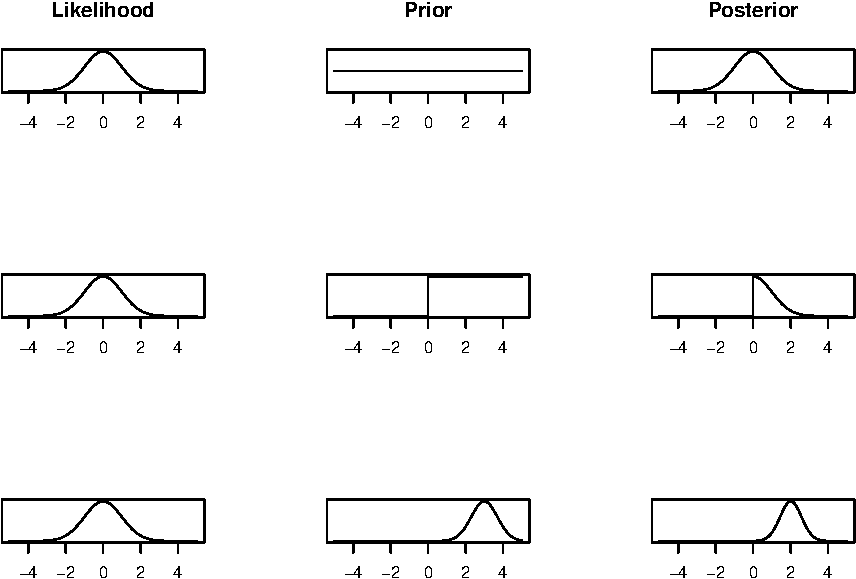
\includegraphics{_main_files/figure-latex/prior-posterior-grid-1.pdf}

\begin{enumerate}
\def\labelenumi{\arabic{enumi}.}
\item
  The posterior distribution is proportional to the likelihood function. The prior distribution closely matches frequentist inference. Both the MLE and posterior mean are 0.
\item
  We get a lopsided posterior distribution, that is proportional to the likelihood function for positive values of \(\theta\), but is 0 for negative values of \(\theta\).
\item
  We get some sort of average of the likelihood function and the prior distribution. Had we collected more data, the posterior distribution would have been weighted toward the information from the likelihood function more.
\end{enumerate}

\end{example}

\hypertarget{programming-in-r}{%
\chapter{Programming in R}\label{programming-in-r}}

\hypertarget{random-numbers-for-loops-and-r}{%
\section{Random Numbers, For Loops and R}\label{random-numbers-for-loops-and-r}}

This first computer lab is about getting used to R. The first step is to download R and Rstudio.

\begin{itemize}
\tightlist
\item
  \href{https://www.r-project.org}{Download R}
\item
  \href{https://posit.co/downloads/}{Download RStudio IDE}
\end{itemize}

The easiest way to learn R is by using it to solve problems. The lab contains four exercises and three ways of approaching the exercise (easy, medium and hard). If you're new to R, use the easy approach and copy and paste the code straight into R -- you'll need to fill in a few blanks though. If you've used R before, or a similar programming language, stick to the medium and hard approaches. This is also an exercise in using Google. Googling around a problem of for specific commands can allow you to quickly find examples (most likely on Stack Overflow) with code you can use.

There are three aims of this lab:

\begin{enumerate}
\def\labelenumi{\arabic{enumi}.}
\tightlist
\item
  Getting used to programming in R.
\item
  Generating random numbers in R.
\item
  \href{https://www.w3schools.com/r/r_for_loop.asp}{Creating for loops in R}.
\end{enumerate}

\begin{example}
Computationally verify that the Poisson distribution with rate \(\lambda = 100\) can be approximated by a normal distribution with mean and variance 100.

To do this, we can generate lots of samples from a Poisson(100) distribution and plot them on top of the density function of the normal distribution with mean and variance 100.

R has four built-in functions for working with distributions. They take the form \texttt{rdist}, \texttt{ddist}, \texttt{pdist}, and \texttt{qdist}. You replace the \texttt{dist} part with the name of the distribution you want to work with, for example \texttt{unif} for the uniform distribution or \texttt{norm} for the normal distribution. As we are working with the the Poisson distribution, we will use \texttt{pois}. The prefixes allow you to work with the distribution in different ways: \texttt{r} gives you random numbers sampled form the distribution, \texttt{d} evaluates the density function, \texttt{p} evaluates the density function, and \texttt{q} evaluates the inverse density function (or quantile function).

The function \texttt{rpois} allows us to generate samples from a Poisson distribution. We store 10,000 samples in a vector \texttt{y} by calling

\begin{Shaded}
\begin{Highlighting}[]
\NormalTok{y }\OtherTok{\textless{}{-}} \FunctionTok{rpois}\NormalTok{(}\AttributeTok{n =} \DecValTok{10000}\NormalTok{, }\AttributeTok{lambda =} \DecValTok{100}\NormalTok{)}
\end{Highlighting}
\end{Shaded}

We can generate a histogram of \texttt{y} using the \texttt{hist} command. Setting \texttt{freq\ =\ FALSE}, makes R plot a density histogram instead of a frequency histogram. Typing \texttt{?hist} will give you more information about this

\begin{Shaded}
\begin{Highlighting}[]
\FunctionTok{hist}\NormalTok{(y, }\AttributeTok{freq =} \ConstantTok{FALSE}\NormalTok{, }\AttributeTok{xlab =} \StringTok{"y"}\NormalTok{, }\AttributeTok{main =} \StringTok{""}\NormalTok{)}
\end{Highlighting}
\end{Shaded}

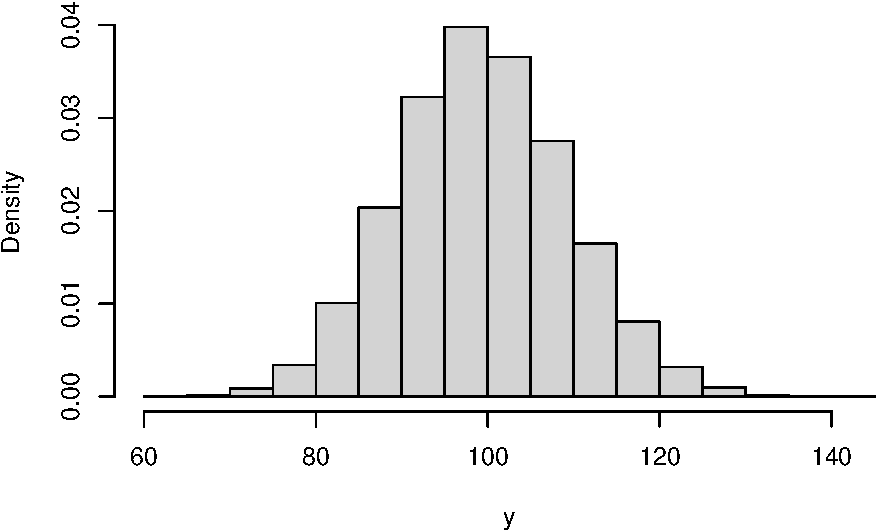
\includegraphics{_main_files/figure-latex/unnamed-chunk-3-1.pdf}

The last thing to do is to plot the normal density on top. There are a couple of ways of doing this. The way below generates a uniform grid of points and then evaluates the density at each point. Finally, it adds a line graph of these densities on top.

\begin{Shaded}
\begin{Highlighting}[]
\NormalTok{x }\OtherTok{\textless{}{-}} \FunctionTok{seq}\NormalTok{(}\AttributeTok{from =} \DecValTok{50}\NormalTok{, }\AttributeTok{to =} \DecValTok{150}\NormalTok{, }\AttributeTok{by =} \DecValTok{1}\NormalTok{)           }\CommentTok{\#create uniform grid on [50, 150]}
\NormalTok{density }\OtherTok{\textless{}{-}} \FunctionTok{dnorm}\NormalTok{(x, }\AttributeTok{mean =} \DecValTok{100}\NormalTok{, }\AttributeTok{sd =} \FunctionTok{sqrt}\NormalTok{(}\DecValTok{100}\NormalTok{)) }\CommentTok{\#compute density}

\CommentTok{\#plot together}
\FunctionTok{hist}\NormalTok{(y, }\AttributeTok{freq =} \ConstantTok{FALSE}\NormalTok{, }\AttributeTok{xlab =} \StringTok{"y"}\NormalTok{, }\AttributeTok{main =} \StringTok{""}\NormalTok{)}
\FunctionTok{lines}\NormalTok{(x, density)}
\end{Highlighting}
\end{Shaded}

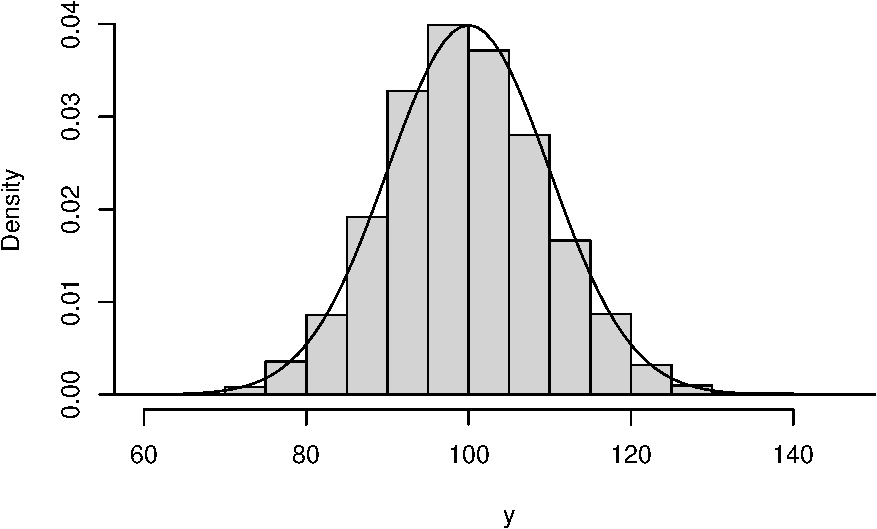
\includegraphics{_main_files/figure-latex/unnamed-chunk-4-1.pdf}

The two match up well, showing the normal distribution is a suitable approximation here.
\end{example}

Over the next two sessions, you will need to solve the following four problems in R. You can type \texttt{?} before any function in R (e.g.~\texttt{?rnorm}) to bring up R's helpage on the function. Googling can also bring up lots of information, possible solutions and support.

\begin{exercise}

The changes in the Birmingham stock exchange each day can be modelled using a normal distribution. The price on day \(i\), \(X_i\) is given by
\[
X_i = \alpha X_{i-1}, \qquad \alpha \sim N(1.001, 0.005^2).
\]
The index begins at \(X_0 = 100\). Investigate the distribution of the value of the stock market on days 50 and 100.

\textbf{Hard}. Use a simulation method to generate the relevant distributions.

\textbf{Medium}. Simulate the value for \(\alpha\) for each of the 100 days and use the \texttt{cumprod} command to plot a trajectory. Use a for loop to repeat this 100 times and investigate the distribution of the value of the stock market on days 50 and 100.

\textbf{Easy}. Fill in the blanks in the following code.

\begin{verbatim}
# Plot one ----------------------------------------------------------------
x <- rnorm(n = , mean = , sd = ) #Simulate daily change for 100 days
plot(, type = 'l') #multiply each day by the previous days

# Plot 100 realisations ---------------------------------------------------
market.index <- matrix(NA, 100, 100) #Initialise a matrix to store trajectories
for(i in 1:100){
  x <- rnorm(n = , mean = , sd = )
  market.index [, i] <- 
}

#Plot all trajectories
matplot(market.index, type = 'l')

#Get distribution of days 50 and 100
hist()
hist()
quantile(, )
quantile(, )
\end{verbatim}

\end{exercise}

\begin{exercise}

You are an avid lottery player and play the lottery twice a week, every week for 50 years (a total of 5,200 times). The lottery has 50 balls labeled 1, \ldots, 50 and you play the same 6 numbers each time. Six out of the 50 balls are chosen uniformly at random and the prize money is shown in the table below.

\begin{longtable}[]{@{}ll@{}}
\toprule\noalign{}
Numbers Matched & Prize Amount \\
\midrule\noalign{}
\endhead
\bottomrule\noalign{}
\endlastfoot
0-2 & £0 \\
3 & £30 \\
4 & £140 \\
5 & £1,750 \\
6 & £1,000,000 \\
\end{longtable}

It costs you £2 to play each time. Simulate one set of 5,200 draws. How much do you win? What is your total profit/loss?

\textbf{Hard}. Use a for loop and sequence of if else statements to generate your prize winnings.

\textbf{Medium}. Use a for loop to generate the lottery numbers and prize winnings for each draw. Use the \texttt{sample} function to generate a set of lottery numbers and check they match against your numbers using the \texttt{\%in\%} function. Finally, use if else statements to check how much you have won each time.

\textbf{Easy}. Fill in the blanks in the following code.

\begin{verbatim}
my.numbers <- 

#For loop to generate lottery numbers and prize winnings
prize <- numeric(5200)
for(i in 1:5200){
  
  #Generate lottery numbers
  draw <- sample(, )
  
  #Check how many match my numbers
  numbers.matched <- #use %in% function
  
  #Compute prize winings
  if(numbers.matched < 3)
    prize[i] <- 0
  else if()
    prize[i] <-  30
  else if()
    prize[i] <-  140
  else if()
    prize[i] <-  1750
  else
    prize[i] <- 1000000
}

#Summarise prize winnings
table(prize)
hist(prize)
sum(prize) - 2*5200
\end{verbatim}

\end{exercise}

\begin{exercise}
Estimate \(\pi\).

\textbf{Hard}. Use a rejection sampling algorithm.

\textbf{Medium}. Generate lots of points \((x, y)\) on the unit square \([0, 1]^2\). Check each point to see if it lies within the unit circle. Use the proportion of points that lie within the unit circle to estimate \(\pi\).

\textbf{Easy}. Fill in the blanks in the following code.

\begin{verbatim}
#Sample on unit square
N <- 10000      #number of points
x <-            #sample N points uniformly at random on [0, 1]
y <-            #sample N points uniformly at random on [0, 1]

#Estimate pi
r.sq                 <- x^2 + y^2                #check how far from origin
number.inside.circle <-           #count how many points inside unit cirlce
pi.estimate          <- 

#Plot points
par(pty = "s")         #make sure plot is square
plot(x, y, cex = 0.1)  #plot points
theta <- seq(0, pi/2, 0.01) #plot unit circle
lines(x = cos(theta), y = sin(theta), col = "red")
\end{verbatim}

\textbf{Extra}. Use a for loop to repeat this for \(N = \{1, \ldots, 10000\}\). Record the estimate for \(\pi\) for each value and the relative error.
\end{exercise}

\begin{exercise}

A linear congruential generator (LCG) is a simple algorithm for generating random integers. Given a starting value \(X_0\), it generates a sequence of integers according to
\[
X_{i+1} = a X_i + c \mod m.
\]
Software that generates numbers using an LCG Setting \(a = 3\), \(c = 2\), \(m = 7\) and \(X_0 = 0\), generate 20 samples from this generator.

\begin{enumerate}
\def\labelenumi{\arabic{enumi}.}
\item
  Investigate the `randomness' of this generator by creating the delay plot, where \(X_{i-1}\) is plotted against \(X_{i}\)
\item
  One way to improve the quality of these generators is to shuffle the sequence generated. Generate rate two sequences \(X\) and \(Y\) from two different LCGs, and report the shuffled sequence \(Z_j = X_{Y_j}\). For the sequence \(Y\) use the values \(a = 5\), \(c = 1\), \(m = 8\) and \(Y_0 = 2\).
\item
  As the past two exercises show, LCGs are notoriously poor. in the 1960s and 70s, RANDU was a widely used LCG developed by IBM. According to Wikipedia
  \textgreater{} IBM's RANDU is widely considered to be one of the most ill-conceived random number generators ever designed, and was described as ``truly horrible'' by Donald Knuth.
\end{enumerate}

The RANDU LCG uses \(a = 2^{16} + 3\), \(c = 0\), \(m = 2^{31}\) and \(Y_0 = 1\). Generate a sequence of 10,000 pseudorandom variables from the RANDU LCG and create the delay plot.

The delay plot seems to show little relationship between \(X_{i}\) and \(X_{i+1}\). The third order delay plot is a 3d-plot with coordinate \((X_i, X_{i+1}, X_{i+2})\) and this plot shows a different picture. Create this plot using the code

\begin{verbatim}
#install.packages("scatterplot3d") #you may need to install this package
scatterplot3d::scatterplot3d(X[1:9998], X[2:9999], X[3:10000], angle=154, 
                             xlab = expression(X[i]), ylab = expression(X[i+1]), zlab = expression(X[i+2]))
\end{verbatim}

This is what makes the RANDU LCG so poor. Write down \(X_{i+1}\) and \(X_{i+2}\) in terms of \(X_i\). Show that \(X_{i+2} = \alpha X_{i+1} + \beta X_{i}\).

\textbf{Hard}. Use a for loop to construct sequences from the LCGs \(X\) and \(Y\).

\textbf{Medium}. Create a for loop to generate the value for the sequence \(X_i\) for \(i = 1, \ldots, 20\). Modular arithmetic can be performed using the \texttt{\%\%} function. Create a new for loop to construct the sequence \(Y\). To shuffle the sequence \(X\) using \(Y\), you will need to subset \(X\) by \(Y\) in R.

\textbf{Easy}. Fill in the blanks in the code below

\begin{verbatim}
# 1. Shuffling ---------------------------------------------------------------
X <- numeric(21) #initialise vector to store X

#Set values for LCG
a <- 
c <- 
m <- 
X[1]<- 


#Run Generator
for(i in 2:21){
  X[i] <-
}
X

#Delay plot
plot( , , xlab = expression(X[i-1]), ylab = expression(X[i]), type = 'l')



# 2. Shuffling ---------------------------------------------------------------

Y <- numeric(21) #initialise vector to store Y

#Set values for LCG
a <- 
c <- 
m <- 
Y[1]<- 


#Run Generator
for(i in 2:50){
  Y[i] <- 
}

#report sequence
Y
X[Y]

#Plot delay plot
plot(x = ,y = , xlab = expression(Z[i-1]), ylab = expression(Z[i]), type = 'l')
\end{verbatim}

\end{exercise}

\hypertarget{functions-in-r}{%
\section{Functions in R}\label{functions-in-r}}

The purpose of this lab is to learn how to write functions is R. Functions are wrappers that allow you to easily repeat commands, as well as customise specific pieces of code.

\hypertarget{built-in-commands}{%
\subsection{Built in commands}\label{built-in-commands}}

R has many build in commands and you used these in Computer Lab I. An example is the \texttt{runif} command from the second exercise. This function generates random numbers from an interval. The code chunk below shows it in action:

\begin{Shaded}
\begin{Highlighting}[]
\NormalTok{u }\OtherTok{\textless{}{-}} \FunctionTok{runif}\NormalTok{(}\AttributeTok{n =} \DecValTok{10}\NormalTok{, }\AttributeTok{min =} \SpecialCharTok{{-}}\DecValTok{1}\NormalTok{, }\AttributeTok{max =} \DecValTok{1}\NormalTok{)}
\NormalTok{u}
\end{Highlighting}
\end{Shaded}

\begin{verbatim}
##  [1]  0.8258991  0.8537517 -0.8580878  0.9768551  0.2945088 -0.2347917
##  [7]  0.3603654  0.7582147 -0.5573377  0.1587472
\end{verbatim}

The functions has three \textbf{arguments}: \emph{n} the number of samples to be generated, \emph{min} the lower limit of the interval, \emph{max} the upper limit of the interval. In the code chunk above 10 random numbers were generated from the interval {[}-1, 1{]}. In R, you don't need to label the arguments, so the following will sample the same number of samples from the same interval:

\begin{verbatim}
u <- runif(10, -1, 1)
\end{verbatim}

Although in most cases it helps to label the arguments for readability and avoiding undefined behaviour. Note that if you decide to omit the argument names in the function call, the arguments must appear exactly in the order defined by the function prototype (check the documentation ?function for specific cases).

\hypertarget{user-defined-functions}{%
\subsection{User defined functions}\label{user-defined-functions}}

In many cases, we will need to repeat the same piece of code over and over again, or we will need to run it again with different values. In this case, we can write our own function. In R, there are two ways to type your own function. The first is to write a full function definition. The basic template is

\begin{verbatim}
name.of.function <- function(arguments){

  #do something
  #produce result
  
  return(result)

}
\end{verbatim}

The second way is an in-line function, which is sometimes useful for short functions. The template is

\begin{verbatim}
name.of.function <- function(arguments) #do something
\end{verbatim}

In this module, we're going to use the full function way of writing functions.

\begin{example}
In this example, we're going to write a function to evaluate the normal density function. The density function is given by
\[
\pi(x \mid \mu, \sigma^2) = \frac{1}{\sqrt{2\pi\sigma^2}}e^{\left\{-\frac{1}{2\sigma^2}(x-\mu)^2\right\}}.
\]

We will need our function to take three arguments, the value at which the density function needs to be evaluated, and the mean and standard deviation of the distribution.

\begin{Shaded}
\begin{Highlighting}[]
\NormalTok{normal.density }\OtherTok{\textless{}{-}} \ControlFlowTok{function}\NormalTok{(x, mu, sigma)\{}
  
\NormalTok{  fraction.term }\OtherTok{\textless{}{-}} \DecValTok{1}\SpecialCharTok{/}\FunctionTok{sqrt}\NormalTok{(}\DecValTok{2}\SpecialCharTok{*}\NormalTok{pi}\SpecialCharTok{*}\NormalTok{sigma}\SpecialCharTok{\^{}}\DecValTok{2}\NormalTok{)}
\NormalTok{  exponent.term }\OtherTok{\textless{}{-}} \SpecialCharTok{{-}}\DecValTok{1}\SpecialCharTok{/}\NormalTok{(}\DecValTok{2}\SpecialCharTok{*}\NormalTok{sigma}\SpecialCharTok{\^{}}\DecValTok{2}\NormalTok{)}\SpecialCharTok{*}\NormalTok{(x}\SpecialCharTok{{-}}\NormalTok{mu)}\SpecialCharTok{\^{}}\DecValTok{2}
  
\NormalTok{  result }\OtherTok{\textless{}{-}}\NormalTok{ fraction.term}\SpecialCharTok{*}\FunctionTok{exp}\NormalTok{(exponent.term)}
  \FunctionTok{return}\NormalTok{(result)}
  
\NormalTok{\}}
\end{Highlighting}
\end{Shaded}

We have split up the density into two parts to make it easier to code up and read. R has its own inbuilt normal density function \texttt{dnorm} and we can compare our function against R's. Although R's is faster and more reliable, we should get the same results.

\begin{Shaded}
\begin{Highlighting}[]
\FunctionTok{normal.density}\NormalTok{(}\AttributeTok{x =} \FloatTok{0.5}\NormalTok{, }\AttributeTok{mu =} \DecValTok{1}\NormalTok{, }\AttributeTok{sigma =} \FloatTok{0.5}\NormalTok{)}
\end{Highlighting}
\end{Shaded}

\begin{verbatim}
## [1] 0.4839414
\end{verbatim}

\begin{Shaded}
\begin{Highlighting}[]
\FunctionTok{dnorm}\NormalTok{(}\AttributeTok{x =} \FloatTok{0.5}\NormalTok{, }\AttributeTok{mean =} \DecValTok{1}\NormalTok{, }\AttributeTok{sd =} \FloatTok{0.5}\NormalTok{)}
\end{Highlighting}
\end{Shaded}

\begin{verbatim}
## [1] 0.4839414
\end{verbatim}

Why might R's function be faster and more reliable than ours?
\end{example}

\begin{exercise}
Write a function to evaluate the log of the probability density function of a Poisson distribution with rate \(\lambda\).
\end{exercise}

\begin{exercise}
Consider the stock exchange problem in Exercise 2.1. Write a function that simulates 100 days of the stock exchange. Use the \texttt{replicate} function to call this function 10,000 times.
\end{exercise}

\hypertarget{good-coding-practices}{%
\section{Good Coding Practices}\label{good-coding-practices}}

In the past two labs, we've written code to solve different problems. In this lab, we're going to take a step back and think about what good R code does and doesn't look like.

\hypertarget{code-style}{%
\subsection{Code Style}\label{code-style}}

Code should be both efficient and easy to read. In most cases it's better to write code that's easy to read and less efficient, than highly efficient code that's difficult to read. Some basic principles to make code easy to read are:

\begin{enumerate}
\def\labelenumi{\arabic{enumi}.}
\tightlist
\item
  Write short functions names, e.g.~\texttt{buy.loot.box} is better than \texttt{player.buys.one.loot.boox} or \texttt{blb}.
\item
  Document and comment code. In R comments start with \texttt{\#}.
\item
  Multiple short functions are better than long functions that do multiple things.
\item
  Be consistent.
\end{enumerate}

\begin{example}
Review the \href{https://style.tidyverse.org/index.html}{tidyverse Style Guide}.
\end{example}

\begin{example}
Review \href{https://google.github.io/styleguide/Rguide.html}{Google's R Style Guide}.
\end{example}

One way to ensure code style is consistent and bug free is to carry out code reviews. These are common both in academia and industry. A code review is where someone else goes through your code line-by-line ensuring it conforms to the company style and doesn't have any bugs.

\begin{exercise}

The following code is for Exercises 2.1 about the stock exchange. Restyle the code so it is easy to read.

\begin{verbatim}
# Plot one ----------------------------------------------------------------
rnorm(100,1.001,0.5) -> x 
plot(100*cumprod(x),type ='l') 
# Plot 100 realisations ---------------------------------------------------
X <- matrix(NA, 100, 100) 
for(i in 1:100){
  x <- rnorm(100, 1.001, 0.005)
  X[,i] <- 100*cumprod(x)
}
matplot(X,type ='l')
hist(X[50,]);hist(X[100,]);quantile(X[50,], c(0.25, 0.5, 0.75));quantile(X[100,], c(0.25, 0.5, 0.75))
\end{verbatim}

\end{exercise}

\begin{exercise}

In pairs or groups, carry out a code review for one of your solutions to an exercise from a previous lab. Remember to

\begin{enumerate}
\def\labelenumi{\arabic{enumi}.}
\tightlist
\item
  Make sure the coding style is consistent.
\item
  Identify any bugs.
\item
  Be respectful and constructive in your feedback.
\end{enumerate}

\end{exercise}

\hypertarget{bayesian-inference}{%
\chapter{Bayesian Inference}\label{bayesian-inference}}

Whereas Chapter 1 dealt with the fundamentals of Bayesian inference and definitions, Chapter 3 is much more practical. We are going to be deriving posterior distributions and proving when it does and doesn't work.

\hypertarget{the-binomial-distribution}{%
\section{The Binomial Distribution}\label{the-binomial-distribution}}

The first example we are going to go through is with the Binomial distribution.

\begin{example}
\protect\hypertarget{exm:binom}{}\label{exm:binom}A social media company wants to determine how many of its users are bots. A software engineer collects a random sample of 200 accounts and finds that eight are bots. She uses a Bayesian method to estimate the probability of an account being a bot. She labels the accounts with a 1 if they are a bot and 0 if there is are a real person. The set of account labels is given by \(\boldsymbol{y} = \{y_1, \ldots, y_{200}\}\) and the probability an account is a bot is \(\theta\). By Bayes' theorem, we obtain the following,
\[
\pi(\theta \mid \boldsymbol{y}) \propto \pi(\boldsymbol{y}\mid \theta) \pi(\theta).
\]

\textbf{Likelihood function} \(\pi(\boldsymbol{y}\mid \theta)\). We observe 200 trials each with the same probability of success (denoted by \(\theta\)) and probability of failure (given by \(1-\theta\)). The Binomial distribution seems the most suitable way of modelling this. Therefore, the likelihood function is given by,
\[
\pi(\boldsymbol{y}\mid \theta) = \begin{pmatrix} 200 \\ 3 \end{pmatrix} \theta^3(1-\theta)^{197},
\]
assuming that any two accounts being a bot are independent of one another.

\textbf{Prior distribution} \(\pi(\theta)\). We now need to describe our prior beliefs about \(\theta\). We have no reason to suggest \(\theta\) takes any specific value, so we use a uniform prior distribution \(\theta \sim U[0, 1]\), where \(\pi(\theta) = 1\) for \(\theta \in [0, 1]\).

\textbf{Posterior distribution} \(\pi(\theta \mid \boldsymbol{y})\). We can now derive the posterior distribution up to proportionality
\[
\pi(\theta \mid \boldsymbol{y}) \propto \theta^3(1-\theta)^{197}. 
\]
This functional dependence on \(\theta\) identifies the \(\pi(\theta \mid \boldsymbol{y})\) is a Beta distribution. The PDF for the beta distribution with shape parameters \(\alpha\) and \(\beta\) is
\[
\pi(x \mid \alpha, \beta) = \frac{\Gamma(\alpha + \beta)}{\Gamma(\alpha)\Gamma(\beta)}x^{\alpha - 1}(1-x)^{\beta - 1}. 
\]
The posterior distribution is therefore \(\theta \mid \boldsymbol{y} \sim \textrm{Beta}(4, 198)\).
\end{example}

\hypertarget{reporting-conclsuions-from-bayesian-inference}{%
\section{Reporting Conclsuions from Bayesian Inference}\label{reporting-conclsuions-from-bayesian-inference}}

In the previous example, we derived the posterior distribution \(\theta \mid \boldsymbol{y} \sim \textrm{Beta}(4, 198)\). But often, we want to share more descriptive information about our beliefs given the observed data. In this example, the posterior mean given the data is \(\frac{4}{198} = \frac{2}{99}\). That is to say given the data, we expect that for every 99 accounts, two to be bots. The posterior mode for \(\theta\) is \(\frac{3}{200}\) or 1.5\%.

It is important to share the uncertainty about out beliefs. In a frequentist framework, this would be via a confidence interval. The Bayesian analogues is a credible interval.

\begin{definition}
A \textbf{credible interval} is a central interval of posterior probability which corresponds, in the case of a 100\((1-\alpha)\)\% interval, to the range of values that capture 100\((1-\alpha)\)\% of the posterior probability.
\end{definition}

\begin{example}
The 95\% credible interval for the Binomial example is given by

\begin{Shaded}
\begin{Highlighting}[]
\NormalTok{cred.int}\FloatTok{.95} \OtherTok{\textless{}{-}} \FunctionTok{qbeta}\NormalTok{(}\FunctionTok{c}\NormalTok{(}\FloatTok{0.025}\NormalTok{, }\FloatTok{0.975}\NormalTok{), }\DecValTok{4}\NormalTok{, }\DecValTok{198}\NormalTok{)}
\FunctionTok{round}\NormalTok{(cred.int}\FloatTok{.95}\NormalTok{, }\DecValTok{3}\NormalTok{)}
\end{Highlighting}
\end{Shaded}

\begin{verbatim}
## [1] 0.005 0.043
\end{verbatim}

This says that we believe there is a 95\% chance that the probability of an account being a bot lies between 0.005 and 0.043. This is a much more intuitive definition to the confidence interval, which says if we ran the experiment an infinite number of times and computed an infinite number of confidence intervals, 95\% of them would contain the true value of \(\theta\).
\end{example}

\hypertarget{the-exponential-distribution}{%
\section{The Exponential Distribution}\label{the-exponential-distribution}}

\begin{example}
\protect\hypertarget{exm:exponential}{}\label{exm:exponential}

An insurance company want to estimate the time until a claim is made on a specific policy. They describe the rate at which claims come in by \(\lambda\). The company provides a sample of 10 months at which a claim was made \(\boldsymbol{y} = \{14, 10, 6, 7, 13, 9, 12, 7, 9, 8\}\). By Bayes' theorem, the posterior distribution for \(\lambda\) is
\[
\pi(\lambda \mid \boldsymbol{y}) \propto \pi(\boldsymbol{y} \mid \lambda) \pi(\lambda).
\]

\textbf{Likelihood function} \(\pi(\boldsymbol{y} \mid \lambda)\). The exponential distribution is a good way of modelling lifetimes or the length of time until an event happens. Assuming all the claims are independent of one another, the likelihood function is given by
\begin{align*}
\pi(\boldsymbol{y} \mid \lambda) &= \prod_{i=1}^{10} \lambda e^{-\lambda y_i} \\
& = \lambda^{10}e^{-\lambda \sum_{i=1}^{10} y_i} \\
& = \lambda^{10} e^{-95\lambda}.
\end{align*}

\textbf{Prior distribution} \(\pi(\lambda)\). As we are modelling a rate parameter, we know it must be positive and continuous. We decide to use an exponential prior distribution for \(\lambda\), but leave the choice of the rate parameter up to the insurance professionals at the insurance company. The prior distribution is given by \(\lambda \sim \textrm{Exp}(\gamma).\)

\textbf{Posterior distribution} \(\pi(\lambda \mid \boldsymbol{y})\). We now have all the ingredients to derive the posterior distribution. It is given by
\begin{align*}
\pi(\lambda \mid \boldsymbol{y}) &\propto \lambda^{10} e^{-95\lambda} \times \lambda e^{-\gamma\lambda} \\
& \propto \lambda^{11}e^{-(95 + \gamma)\lambda}
\end{align*}
The functional form tells us that the posterior distribution is a Gamma distribution. The PDF of a gamma random variable with shape \(\alpha\) and rate \(\beta\) is
\[
\pi(x \mid \alpha, \beta) = \frac{\alpha^\beta}{\Gamma(\alpha)}x^{\alpha-1}e^{-\beta x}.
\]
The distribution of the rate of the claims given the observed data is \(\lambda \mid \boldsymbol{y} \sim \textrm{Gamma}(10, 95 + \gamma)\).

The posterior mean months until a claim is \(\frac{10}{95 + \gamma}\). We can see the effect of the choice of rate parameter in this mean. Small values of \(\gamma\) yield vague prior distribution, which plays a minimal role in the posterior distribution. Large values of \(\gamma\) result in prior distributions that contribute a lot to the posterior distribution. The plots below show the prior and posterior distributions for \(\gamma = 0.01\) and \(\gamma = 50\).

\begin{Shaded}
\begin{Highlighting}[]
\NormalTok{plot.distributions }\OtherTok{\textless{}{-}} \ControlFlowTok{function}\NormalTok{(gamma.prior)\{}
  \CommentTok{\#evaluate at selected values of theta}
\NormalTok{  theta }\OtherTok{\textless{}{-}} \FunctionTok{seq}\NormalTok{(}\FloatTok{0.001}\NormalTok{, }\FloatTok{0.3}\NormalTok{, }\FloatTok{0.001}\NormalTok{) }
  
  \CommentTok{\#evaluate prior density}
\NormalTok{  prior }\OtherTok{\textless{}{-}} \FunctionTok{dexp}\NormalTok{(theta, }\AttributeTok{rate =}\NormalTok{ gamma.prior)}
  
  \CommentTok{\#evaluate posterior density}
\NormalTok{  posterior }\OtherTok{\textless{}{-}} \FunctionTok{dgamma}\NormalTok{(theta, }\AttributeTok{shape =} \DecValTok{10}\NormalTok{, }\AttributeTok{rate =} \DecValTok{95} \SpecialCharTok{+}\NormalTok{ gamma.prior)}
  
  
  \CommentTok{\#plot}
  \FunctionTok{plot}\NormalTok{(theta, posterior, }\AttributeTok{type=} \StringTok{\textquotesingle{}l\textquotesingle{}}\NormalTok{, }
       \AttributeTok{ylim =} \FunctionTok{c}\NormalTok{(}\DecValTok{0}\NormalTok{, }\DecValTok{50}\NormalTok{), }\AttributeTok{xlab =} \FunctionTok{expression}\NormalTok{(theta), }\AttributeTok{ylab =} \StringTok{"density"}\NormalTok{)}
  \FunctionTok{lines}\NormalTok{(theta, prior, }\AttributeTok{lty =} \DecValTok{2}\NormalTok{)}
  \FunctionTok{legend}\NormalTok{(}\StringTok{\textquotesingle{}topright\textquotesingle{}}\NormalTok{, }\AttributeTok{lty =} \FunctionTok{c}\NormalTok{(}\DecValTok{1}\NormalTok{, }\DecValTok{2}\NormalTok{), }\AttributeTok{legend =} \FunctionTok{c}\NormalTok{(}\StringTok{"Posterior"}\NormalTok{, }\StringTok{"Prior"}\NormalTok{),  }
         \AttributeTok{bty =} \StringTok{"n"}\NormalTok{)}
\NormalTok{\}}

\FunctionTok{plot.distributions}\NormalTok{(}\FloatTok{0.01}\NormalTok{)}
\end{Highlighting}
\end{Shaded}

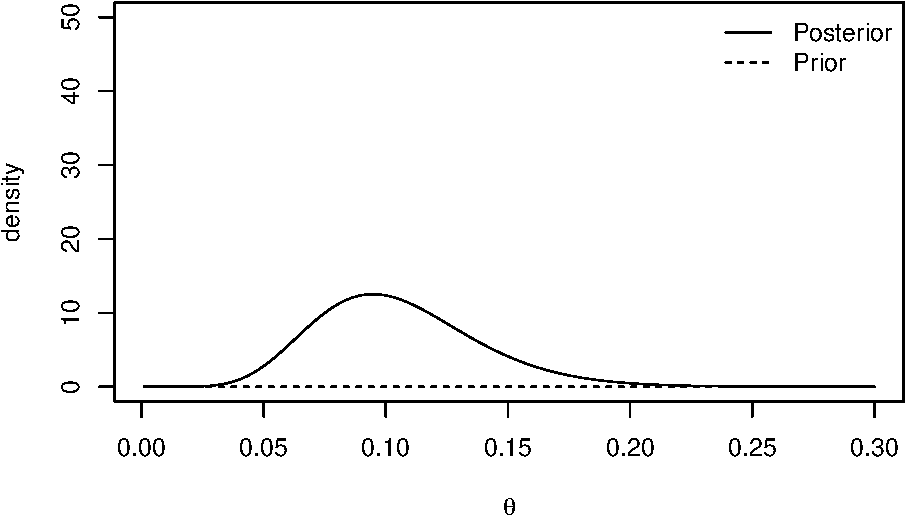
\includegraphics{_main_files/figure-latex/unnamed-chunk-9-1.pdf}

\begin{Shaded}
\begin{Highlighting}[]
\FunctionTok{plot.distributions}\NormalTok{(}\DecValTok{50}\NormalTok{)}
\end{Highlighting}
\end{Shaded}

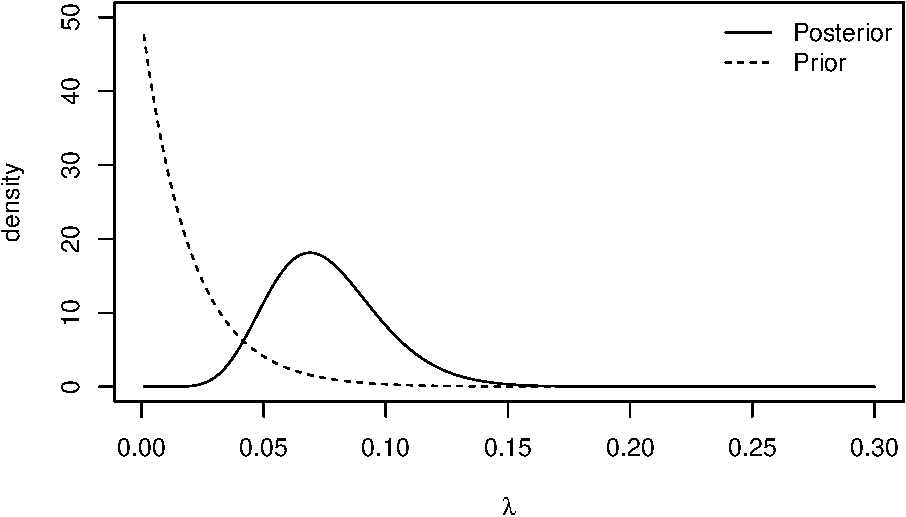
\includegraphics{_main_files/figure-latex/unnamed-chunk-9-2.pdf}

The insurance managers recommend that because this is a new premium, a vague prior distribution be used and \(\gamma = 0.01\). The posterior mean is \(\frac{10}{95.01} \approx 0.105\) and the 95\% credible interval is

\begin{Shaded}
\begin{Highlighting}[]
\FunctionTok{round}\NormalTok{(}\FunctionTok{qgamma}\NormalTok{(}\FunctionTok{c}\NormalTok{(}\FloatTok{0.025}\NormalTok{, }\FloatTok{0.975}\NormalTok{), }\DecValTok{10}\NormalTok{, }\FloatTok{95.01}\NormalTok{), }\DecValTok{3}\NormalTok{)}
\end{Highlighting}
\end{Shaded}

\begin{verbatim}
## [1] 0.05 0.18
\end{verbatim}

\end{example}

\hypertarget{the-normal-distribtuion}{%
\section{The Normal Distribtuion}\label{the-normal-distribtuion}}

The Normal distribution is incredibly useful for modelling a wide range of natural phenomena and in its own right. We're now going to derive posterior distributions for the normal distribution. As we're going to see, the concepts behind deriving posterior distributions are the same as in the previous two examples. However, the algebraic accounting is a lot more taxing.

\begin{example}
\protect\hypertarget{exm:normal}{}\label{exm:normal}

Suppose we observe \(N\) data points \(\boldsymbol{y} = \{y_1, \ldots, y_N\}\) and we assume \(y_i \sim N(\mu, \sigma^2)\) and each observation is independent. Suppose that, somehow, we know the population standard deviation and we wish to estimate the population mean \(\mu\). By Bayes' theorem, the posterior distribution is
\[
\pi(\mu \mid \boldsymbol{y}, \sigma^2) \propto \pi(\boldsymbol{y} \mid \mu, \sigma^2) \pi(\mu)
\]

\textbf{Likelihood function}.
As the observations are independent, the likelihood function is given by the product of the \(N\) normal density functions as follows,
\begin{align*}
\pi(\boldsymbol{y} \mid \mu, \theta^2) &= \prod_{i=1}^{N} \frac{1}{\sqrt{2\pi\sigma^2}}\exp\left\{-\frac{(y_i - \mu)^2}{2\sigma^2}\right\} \\
&= (2\pi\sigma^2)^{-\frac{N}{2}}\exp\left\{-\sum_{i=1}^{N}\frac{(y_i - \mu)^2}{2\sigma^2}\right\}.
\end{align*}

\textbf{Prior distribution} We suppose we have no prior beliefs about the values that \(\mu\) can take. We assign a normal prior distribution to \(\mu \sim N(\mu_0, \sigma_0^2)\) despite it being a time. We will set \(\mu = 0\) and \(\sigma_0^2 = 1000\) to signify our vague prior beliefs, but, for ease, we will use the symbolic values during the derivation of the posterior distribution. We have
\[
\pi(\mu) = \frac{1}{\sqrt{2\pi\sigma_0^2}}\exp\left\{-\frac{1}{2\sigma_0^2}(\mu - \mu_0)^2\right\}.
\]

\textbf{Posterior distribution}. To derive the posterior distribution, up to proportionality, we multiply the prior distribution by the likelihood function. As the fractions out the front of both terms do not depend on \(\mu\), we can ignore these.
\begin{align*}
\pi(\mu \mid \boldsymbol{y}, \sigma^2) &\propto\exp\left\{-\sum_{i=1}^{N}\frac{(y_i - \mu)^2}{2\sigma^2}\right\}  \exp\left\{\frac{1}{2\sigma_0^2}(\mu - \mu_0)^2\right\} \\
& = \exp\left\{-\sum_{i=1}^{N}\frac{(y_i - \mu)^2}{2\sigma^2}-\frac{1}{2\sigma_0^2}(\mu - \mu_0)^2\right\} \\
& = \exp\left\{-\frac{\sum_{i=1}^{N}y_i^2}{2\sigma^2} + \frac{\mu\sum_{i=1}^{N}y_i}{\sigma^2} - \frac{N\mu^2}{2\sigma^2} - \frac{\mu^2}{2\sigma_0^2} + \frac{\mu\mu_0}{\sigma_0^2} - \frac{\mu_0^2}{2\sigma_0^2}\right\}.
\end{align*}

We can drop the first and last term as they do not depend on \(\mu\). With some arranging, the equation becomes
\[
\pi(\mu \mid \boldsymbol{y}, \sigma^2) \propto \exp\left\{-\mu^2\left(\frac{N}{2\sigma^2}  + \frac{1}{2\sigma_0^2}\right) + \mu\left(\frac{\sum_{i=1}^{N}y_i}{\sigma^2} + \frac{\mu_0}{\sigma_0^2} \right)  \right\}
\]
Defining \(\mu_1 =\left(\frac{\sum_{i=1}^{N}y_i}{\sigma^2} + \frac{\mu_0}{\sigma_0^2} \right)\) and \(\sigma^2_1 = \left(\frac{N}{\sigma^2} + \frac{1}{\sigma_0^2}\right)^{-1}\) tidies this up and gives
\[
\pi(\mu \mid \boldsymbol{y}, \sigma^2) \propto \exp\left\{-\frac{\mu^2}{2\sigma_1^2} + \mu\mu_1 \right\}.
\]
Our last step to turning this into a distribution is completing the square. Consider the exponent term, completing the square becomes
\[
-2\sigma_1^2\mu^2 + \mu\mu_1 = -\frac{1}{2\sigma^2_1}\left(\mu - \frac{\mu_1}{\sigma_1^2} \right)^2.
\]
Therefore, the posterior distribution, up to proportionality, is given by
\[
\pi(\mu \mid \boldsymbol{y}, \sigma^2) \propto \exp\left\{-\frac{1}{2\sigma^2_1}\left(\mu - \frac{\mu_1}{\sigma_1^2} \right)^2\right\},
\]
and so the posterior distribution of \(\mu\) is \(\mu \mid \boldsymbol{y}, \sigma^2 \sim N(\mu_1, \sigma^2_1)\).

It may help to consider the meaning of \(\mu_1\) and \(\sigma^2_1\). The variance of the posterior distribution can be thought of as the weighted average of the population and sample precision, where the weight is the number of data points collected. The interpretation of the posterior mean can be seen more easily by writing is as
\[
\mu  = \sigma_1^2\left(\frac{N\bar{y}}{\sigma^2} + \frac{\mu_0}{\sigma_0^2} \right).
\]
The posterior mean is partially defined through the weighted average of the population and prior means, where the weighting depends on the number of data points collected and how precise the distributions are.

Now we have derived the posterior distribution, we can explore it using R. We simulate some data with \(N = 30\), \(mu = 5\) and \(\sigma^2 = 1\).

\begin{Shaded}
\begin{Highlighting}[]
\CommentTok{\#data}
\NormalTok{N }\OtherTok{\textless{}{-}} \DecValTok{30}
\NormalTok{sigma }\OtherTok{\textless{}{-}} \DecValTok{1}
\NormalTok{y }\OtherTok{\textless{}{-}} \FunctionTok{rnorm}\NormalTok{(N, }\DecValTok{5}\NormalTok{, sigma)}

\CommentTok{\#prior}
\NormalTok{sigma0 }\OtherTok{\textless{}{-}} \DecValTok{1000}
\NormalTok{mu0     }\OtherTok{\textless{}{-}} \DecValTok{0}

\CommentTok{\#posterior}
\NormalTok{sigma1.sq }\OtherTok{\textless{}{-}}\NormalTok{ (}\DecValTok{1}\SpecialCharTok{/}\NormalTok{(sigma0}\SpecialCharTok{\^{}}\DecValTok{2}\NormalTok{)  }\SpecialCharTok{+}\NormalTok{ N}\SpecialCharTok{/}\NormalTok{(sigma}\SpecialCharTok{\^{}}\DecValTok{2}\NormalTok{))}\SpecialCharTok{\^{}{-}}\DecValTok{1}
\NormalTok{mu1       }\OtherTok{\textless{}{-}}\NormalTok{ sigma1.sq}\SpecialCharTok{*}\NormalTok{(}\FunctionTok{sum}\NormalTok{(y)}\SpecialCharTok{/}\NormalTok{(sigma}\SpecialCharTok{\^{}}\DecValTok{2}\NormalTok{) }\SpecialCharTok{+}\NormalTok{ mu0}\SpecialCharTok{/}\NormalTok{(sigma0}\SpecialCharTok{\^{}}\DecValTok{2}\NormalTok{))}

\FunctionTok{c}\NormalTok{(mu1, sigma1.sq) }\CommentTok{\#output mean and variance}
\end{Highlighting}
\end{Shaded}

\begin{verbatim}
## [1] 5.08969873 0.03333333
\end{verbatim}

\begin{Shaded}
\begin{Highlighting}[]
\CommentTok{\#Create plot}
\NormalTok{mu }\OtherTok{\textless{}{-}} \FunctionTok{seq}\NormalTok{(}\DecValTok{4}\NormalTok{, }\DecValTok{6}\NormalTok{, }\FloatTok{0.01}\NormalTok{)}
\NormalTok{posterior }\OtherTok{\textless{}{-}} \FunctionTok{dnorm}\NormalTok{(mu, }\AttributeTok{mean =}\NormalTok{ mu1, }\AttributeTok{sd =} \FunctionTok{sqrt}\NormalTok{(sigma1.sq))}
\FunctionTok{plot}\NormalTok{(mu, posterior, }\AttributeTok{type =}\StringTok{\textquotesingle{}l\textquotesingle{}}\NormalTok{)}
\end{Highlighting}
\end{Shaded}

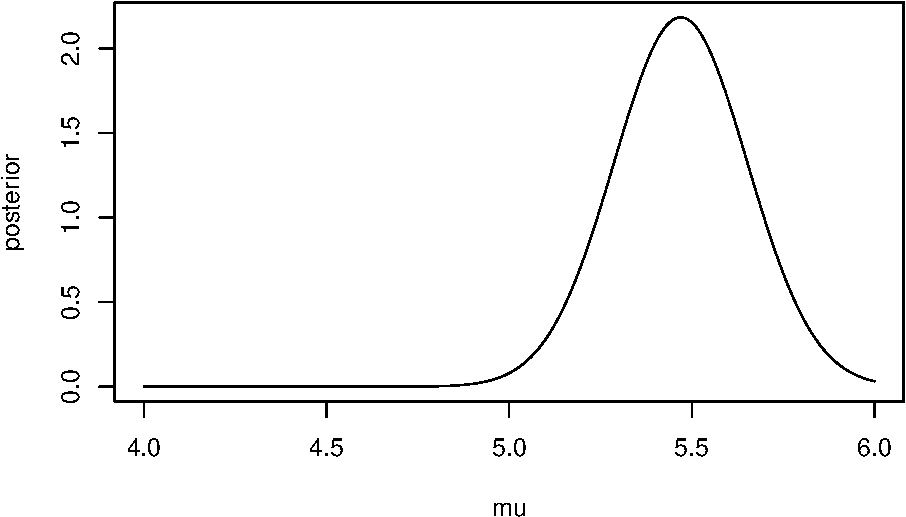
\includegraphics{_main_files/figure-latex/unnamed-chunk-11-1.pdf}

The 95\% credible interval for the population's mean reaction time is

\begin{Shaded}
\begin{Highlighting}[]
\FunctionTok{qnorm}\NormalTok{(}\FunctionTok{c}\NormalTok{(}\FloatTok{0.025}\NormalTok{, }\FloatTok{0.975}\NormalTok{), mu1, }\FunctionTok{sqrt}\NormalTok{(sigma1.sq))}
\end{Highlighting}
\end{Shaded}

\begin{verbatim}
## [1] 4.731860 5.447538
\end{verbatim}

\end{example}

When the prior distribution induces the same function form in the posterior distribution, this is known as conjugacy.

If the prior distribution \(\pi(\theta)\) has the same distributional family as the posterior distribution \(\pi(\theta \mid \boldsymbol{y})\), then the prior distribution is a \textbf{conjugate prior distribution}.

\hypertarget{hierarchical-models}{%
\section{Hierarchical Models}\label{hierarchical-models}}

In many modelling problems, there will be multiple parameters each related to one another. These parameters may be directly related to the model, or they may be parameters we introduce through prior distributions. We can form a hierarchy of these parameters, from closest to further from the data, to construct our model.

\begin{example}
Let's consider \ref{exm:exponential} again. We have some data \(\boldsymbol{y}\) that are assumed to have been generated from an Exponential distribution with rate parameter \(\lambda\). We placed an Exponential prior distribution with rate \(\gamma\) on \(\lambda\) and the posterior distribution was \(\lambda \mid \boldsymbol{y} \sim \textrm{Gamma}(10, 95 + \gamma)\).

In that example, we discussed how the choice of \(\gamma\) can affect the posterior distribution and conclusions presented to the company. One option is to place a prior distribution on \(\gamma\) -- a hyperprior distribution. The hierachy formed is
\begin{align*}
\boldsymbol{y} \mid \lambda &\sim \hbox{Exp}(\lambda) & \textrm{(likelihood)} \\
\lambda \mid \gamma &\sim \hbox{Exp}(\gamma) & \textrm{(prior distribution)} \\
\gamma \mid \nu &\sim \hbox{Exp}(\nu) & \textrm{(hyperprior distribution)}  \\
\end{align*}.
By Bayes' theorem, we can write the posterior distribution as
\begin{align*}
\pi(\lambda, \gamma \mid \boldsymbol{y}) \propto \pi(\boldsymbol{y} \mid \lambda)\pi(\lambda \mid \gamma)\pi(\gamma)\\
&\propto \lambda^{11}e^{-\lambda(95 + \gamma)}\nu e^{-\nu\gamma}.
\end{align*}

To derive the full conditional distributions, we only consider the terms that depends on the parameters we are interested in. The full conditional distribution for \(\lambda\) is
\[
\pi(\lambda \mid \boldsymbol{y}, \,\gamma) \propto \lambda^{11}e^{-\lambda(95 + \gamma)}.
\]
This is unchanged and shows that \(\lambda \mid \boldsymbol{y}, \gamma \sim \textrm{Gamma}(10, 95 + \gamma)\). The full conditional distribution for \(\gamma\) is
\[
\pi(\gamma \mid \boldsymbol{y}, \,\lambda) \propto e^{-\nu\gamma}.
\]
Therefore the full conditional distribution of \(\gamma\) is \(\gamma \mid \boldsymbol{y}, \,\lambda \sim \hbox{Exp}(\lambda + \nu)\).
In the next chapter, we will look at how to sample from these distributions.
\end{example}

\hypertarget{prediction}{%
\section{Prediction}\label{prediction}}

In many cases, although we are interested in drawing inference for the model parameters, what we may also be interested in is predicting new values, whose distribution is determined by the model parameters and observed data.

\begin{definition}
Suppose we observe some data \(\boldsymbol{y}\) given some model parameters \(\theta\) and assign a prior distribution to \(\theta\) and hence derive the posterior distribution \(\pi(\theta \mid \boldsymbol{y})\). The quantity we are interested in is some future observation \(z\), we would like to the distribution of \(z\) given the observed data \(\boldsymbol{y}\), denoted by \(\pi(z \mid \boldsymbol{y})\). This distribution, known as the \textbf{posterior predictive distribution} of \(z\) must be exhibited as a mixture distribution over the possible values of \(\theta\) and is written as,
\[
\pi(z \mid \boldsymbol{y}) = \int \pi(z \mid \theta) \pi(\theta \mid \boldsymbol{y})\, d\theta.
\]
\end{definition}

\begin{example}

Students have to submit coursework for a particular statistical modules. However, each semester a number of students miss the deadline and hand in their coursework late. Last year, three out of 20 students handed their coursework in late. This year, the course has thirty students in. How many students can we expect to hand in their coursework late?

We can model the number of students handing their coursework in late, denoted by \(Y\), using a Binomial distribution, i.e.~\(Y \sim \textrm{Bin}(n, \theta)\) where \(n\) is the number of students and \(\theta\) is the probability of any particular student handing in their coursework late. As in Example \ref{exm:binom}, we assign a uniform prior distribution to \(\theta \sim U[0, 1]\). Given then observed data, we can derive \(\theta \mid \boldsymbol{y} \sim Beta(4, 28)\) (See problem sheets for derivation).

Now we can derive the posterior predictive distribution of \(Z\), the number of students who hand in late. We model \(Z\) using a Binomial distribution, \(Z \sim \textrm{Bin}(30, \theta)\). The distribution of \(Z\) given the observed data is

\begin{align*}
\pi(z \mid \boldsymbol{y}) &= \int_0^1 \pi(z \mid \theta) \pi(\theta \mid \boldsymbol{y})\, d\theta \\
& = \int_0^1 \begin{pmatrix} 30 \\ z \end{pmatrix} \theta^z (1-\theta)^{30 - z} \frac{\Gamma(32)}{\Gamma(4)\Gamma(28)}\theta^{3}(1-\theta)^{27}\, d\theta \\
 & = \begin{pmatrix} 30 \\ z \end{pmatrix}\frac{\Gamma(32)}{\Gamma(4)\Gamma(28)}\int_0^1 \theta^{z + 3}(1-\theta)^{57 - z}\, d\theta \\
\end{align*}
This integral is difficult to evaluate immediately. But by multiplying (and dividing outside the integral) by a constant, we can turn it into the density function of a Beta\((5 + z, 58 - z)\) random variable. This integrates to 1.

\begin{align*}
\pi(z \mid \boldsymbol{y})  & = \begin{pmatrix} 30 \\ z \end{pmatrix}\frac{\Gamma(32)}{\Gamma(4)\Gamma(28)}\frac{\Gamma(z+4)\Gamma(58-z)}{\Gamma(62)}\int_0^1 \frac{\Gamma(62)}{\Gamma(z+4)\Gamma(58-z)}\theta^{z + 3}(1-\theta)^{57 - z}\, d\theta \\ 
& = \begin{pmatrix} 30 \\ z \end{pmatrix}\frac{\Gamma(32)\Gamma(z+4)\Gamma(58-z)}{\Gamma(4)\Gamma(28)\Gamma(62)} \quad \textrm{for }  z \in \{0,1,...,30 \}.
\end{align*}

This code implements the distribution

\begin{Shaded}
\begin{Highlighting}[]
\NormalTok{beta.binom.posterior.predictive.distribution }\OtherTok{\textless{}{-}} \ControlFlowTok{function}\NormalTok{(z)\{}
  
  
\NormalTok{  numerator }\OtherTok{\textless{}{-}} \FunctionTok{gamma}\NormalTok{(}\DecValTok{32}\NormalTok{)}\SpecialCharTok{*}\FunctionTok{gamma}\NormalTok{(z }\SpecialCharTok{+} \DecValTok{4}\NormalTok{)}\SpecialCharTok{*}\FunctionTok{gamma}\NormalTok{(}\DecValTok{58}\SpecialCharTok{{-}}\NormalTok{z)}
\NormalTok{  denominator }\OtherTok{\textless{}{-}} \FunctionTok{gamma}\NormalTok{(}\DecValTok{4}\NormalTok{)}\SpecialCharTok{*}\FunctionTok{gamma}\NormalTok{(}\DecValTok{28}\NormalTok{)}\SpecialCharTok{*}\FunctionTok{gamma}\NormalTok{(}\DecValTok{62}\NormalTok{)}
  
\NormalTok{  output }\OtherTok{\textless{}{-}} \FunctionTok{choose}\NormalTok{(}\DecValTok{30}\NormalTok{, z)}\SpecialCharTok{*}\NormalTok{numerator}\SpecialCharTok{/}\NormalTok{denominator}
  \FunctionTok{return}\NormalTok{(output)}
  
\NormalTok{\}}
\end{Highlighting}
\end{Shaded}

We can check that our posterior predictive distribution is a valid probability mass function by checking that the probabilities sum to one.

\begin{Shaded}
\begin{Highlighting}[]
\NormalTok{z }\OtherTok{\textless{}{-}} \DecValTok{0}\SpecialCharTok{:}\DecValTok{30}
\NormalTok{ppd }\OtherTok{\textless{}{-}} \FunctionTok{beta.binom.posterior.predictive.distribution}\NormalTok{(z)}
\FunctionTok{sum}\NormalTok{(ppd)}
\end{Highlighting}
\end{Shaded}

\begin{verbatim}
## [1] 1
\end{verbatim}

\begin{Shaded}
\begin{Highlighting}[]
\FunctionTok{plot}\NormalTok{(z, ppd, }\AttributeTok{xlab =} \StringTok{"z"}\NormalTok{, }\AttributeTok{ylab =} \StringTok{"Posterior predictive mass"}\NormalTok{)}
\end{Highlighting}
\end{Shaded}

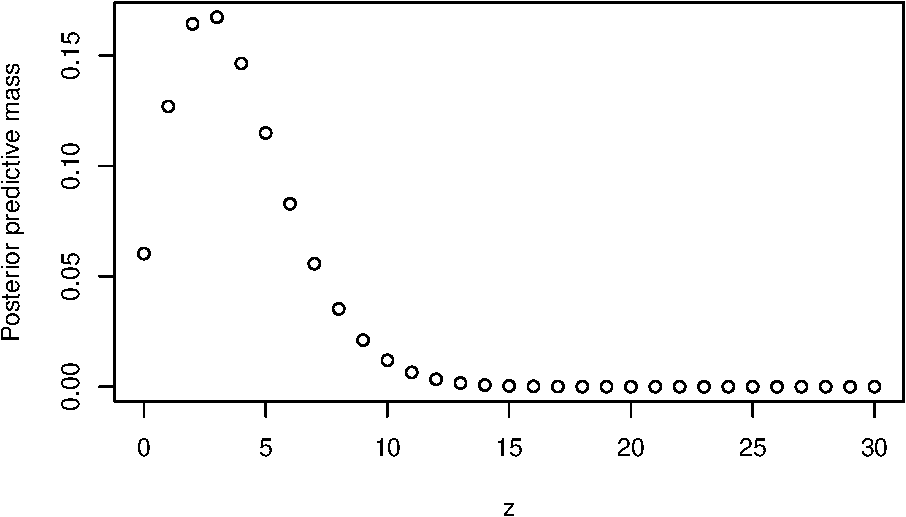
\includegraphics{_main_files/figure-latex/unnamed-chunk-14-1.pdf}

The expected number of students who hand in late is 3.75 and there's a 95\% chance that up to 8 hand in late.

\begin{Shaded}
\begin{Highlighting}[]
\NormalTok{z}\SpecialCharTok{\%*\%}\NormalTok{ppd }\CommentTok{\#expectation}
\end{Highlighting}
\end{Shaded}

\begin{verbatim}
##      [,1]
## [1,] 3.75
\end{verbatim}

\begin{Shaded}
\begin{Highlighting}[]
\FunctionTok{cbind}\NormalTok{(z, }\FunctionTok{cumsum}\NormalTok{(ppd)) }\CommentTok{\#CDF}
\end{Highlighting}
\end{Shaded}

\begin{verbatim}
##        z           
##  [1,]  0 0.06029453
##  [2,]  1 0.18723037
##  [3,]  2 0.35156696
##  [4,]  3 0.51889148
##  [5,]  4 0.66530044
##  [6,]  5 0.78021765
##  [7,]  6 0.86309065
##  [8,]  7 0.91880359
##  [9,]  8 0.95404202
## [10,]  9 0.97513714
## [11,] 10 0.98713498
## [12,] 11 0.99363285
## [13,] 12 0.99698773
## [14,] 13 0.99863936
## [15,] 14 0.99941423
## [16,] 15 0.99976022
## [17,] 16 0.99990696
## [18,] 17 0.99996591
## [19,] 18 0.99998826
## [20,] 19 0.99999622
## [21,] 20 0.99999887
## [22,] 21 0.99999969
## [23,] 22 0.99999992
## [24,] 23 0.99999998
## [25,] 24 1.00000000
## [26,] 25 1.00000000
## [27,] 26 1.00000000
## [28,] 27 1.00000000
## [29,] 28 1.00000000
## [30,] 29 1.00000000
## [31,] 30 1.00000000
\end{verbatim}

\end{example}

\hypertarget{non-informative-prior-distibrutions}{%
\section{Non-informative Prior Distibrutions}\label{non-informative-prior-distibrutions}}

We have seen in a few examples how the choice of the prior distribution (and prior parameters) can impact posterior distributions and the resulting conclusions. As the choice of prior distribution is subjective, it is the main criticism of Bayesian inference. A possible way around this is to use a prior distribution that reflects a lack of information about \(\theta\).

\begin{definition}
A \textbf{non-informative prior distribution} is a prior distribution that places equal weight on the every possible value of \(\theta\).
\end{definition}

\begin{example}
In Example \ref{exm:binom}, we assigned a uniform prior distribution to the parameter \(\theta\).
\end{example}

Such a prior distribution can have interesting and perhaps unintended side effects. Suppose we do indeed have some parameter \(\theta\) and we place a uniform prior distribution on \(\theta\) such that \(\theta \sim U[0, 1]\). This means, for example, our prior beliefs about \(\theta\) are that it is equally likely to be in \([0, 0.1]\) as it is to lie in \([0.8, 0.9]\) or any other interval of size 0.1. However, our prior beliefs about \(\theta^2\) are not uniform. Letting \(\phi = \theta^2\), changing variables gives \(\pi(\phi) = \frac{1}{2\sqrt{\phi}}\), something that is not uniform. That raises the question, if we have little to say about \(\theta\) \textit{a priori}, shouldn't we have little to say about any reasonable transformation of \(\theta\)?

\begin{theorem}[Jeffrey]
Given some observed data \(\boldsymbol{y} = \{y_1, \ldots, y_N\}\), an invariant prior distribution is
\[
\pi(\theta) \propto \sqrt{I_\theta(\boldsymbol{y})},
\]
where \(I_\theta(\boldsymbol{y})\) is the Fisher information for \(\theta\) contained in \(\boldsymbol{y}\).
\end{theorem}

Jeffrey argues that if there are two ways of parameterising a model, e.g.~via \(\theta\) and \(\psi\), then the priors on these parameters should be equivalent. In other words, the prior distribution should be invariant under sensible (one-to-one) transformations.

\begin{proof}
Recall that the distribution of \(\psi = h(\theta)\), for some one-to-one function \(h\), is invariant to the distribution of \(\theta\) if
\[
\pi(\psi) = \pi(\theta) \left|\frac{d\theta}{d\psi}\right|.
\]
Transforming the Fisher information for \(\psi\) shows
\begin{align*}
I_\psi(\boldsymbol{y}) &= - \mathbb{E}\left(\frac{d^2\log \pi(\boldsymbol{y} \mid \psi)}{d\psi^2}\right) \\
& = \mathbb{E}\left(\frac{d^2 \log \pi(\boldsymbol{y} \mid \theta = h^{-1}(\psi))}{d\theta^2}\right) \left(\frac{d\theta}{d\psi}\right)^2 \\
& = I_\theta(\boldsymbol{y})\left(\frac{d\theta}{d\psi}\right)^2 .
\end{align*}
Thus \(\sqrt{I_\psi(\boldsymbol{y})} = \sqrt{I_\theta(\boldsymbol{y})} \left|\frac{d\theta}{d\psi}\right|\) and \(\sqrt{I_\psi(\boldsymbol{y})}\) and \(\sqrt{I_\theta(\boldsymbol{y})}\) are invariant prior distributions.
\end{proof}

\begin{example}
In Example \ref{exm:binom}, we modelled the number of bot accounts on a social media website by \(Y \sim \textrm{Bin}(n, \theta)\). To construct Jeffrey's prior distribution for \(\theta\), we must first derive the Fisher information.\\
\begin{align*}
&\pi(y \mid \theta) = \begin{pmatrix} n \\ y \end{pmatrix} \theta^y (1-\theta)^{n-y}\\ 
\implies &\log \pi(y \mid \theta) = \log \begin{pmatrix} n \\ y \end{pmatrix} + y \log\theta + (n-y)\log(1-\theta) \\
\implies &\frac{\partial \log \pi(y \mid \theta)}{\partial \theta} = \frac{y}{\theta} - \frac{n-y}{1-\theta} \\
\implies &\frac{\partial^2 \log \pi(y \mid \theta)}{\partial \theta^2} = -\frac{y}{\theta^2} + \frac{n-y}{(1-\theta)^2} \\
\implies &\mathbb{E}\left(\frac{\partial \log \pi(y \mid \theta)}{\partial \theta}\right) = -\frac{\mathbb{E}(y)}{\theta^2} + \frac{n-\mathbb{E}(y)}{(1-\theta)^2}\\ 
\implies &\mathbb{E}\left(\frac{\partial \log \pi(y \mid \theta)}{\partial \theta}\right) = -\frac{n\theta}{\theta^2} + \frac{n-n\theta}{(1-\theta)^2}\\ 
\implies &\mathbb{E}\left(\frac{\partial \log \pi(y \mid \theta)}{\partial \theta}\right) = -\frac{n}{\theta} + \frac{n}{1-\theta}\\
\implies &\mathbb{E}\left(\frac{\partial \log \pi(y \mid \theta)}{\partial \theta}\right) = -\frac{n}{\theta(1-\theta)} \\
\implies &I_\theta(y) \propto \frac{1}{\theta(1-\theta)}.
\end{align*}

Hence Jeffrey's prior is \(\pi(\theta) \propto \theta^{-\frac{1}{2}}(1-\theta)^{-\frac{1}{2}}\). This functional dependency on \(\theta\) shows that \(\theta \sim \textrm{Beta}(\frac{1}{2}, \frac{1}{2})\).
\end{example}

\hypertarget{bernstein-von-mises-theorem}{%
\section{Bernstein-von-Mises Theorem}\label{bernstein-von-mises-theorem}}

So far, we have considered Bayesian methods in contrast to frequentist ones. The Bernstein-von-Mises theorem is a key theorem linking the two inference methods.

\begin{theorem}[Bernstein-von-Mises]
For a well-specified model \(\pi(\boldsymbol{y} \mid \theta)\) with a fixed number of parameters, and for a smooth prior distribution \(\pi(\theta)\) that is non-zero around the MLE \(\hat{\theta}\), then
\[
\left|\left| \pi(\theta \mid \boldsymbol{y}) - N\left(\hat{\theta}, \frac{I(\hat{\theta})^{-1}}{n}\right) \right|\right|_{TV} \rightarrow 0,
\]
where \(||p - q||_{TV}\) is the total variation distance between distributions \(p\) and \(q\):
\[
||p - q||_{TV} = \frac{1}{2}\int|\pi(x) - q(x)|\,dx.
\]
\end{theorem}

The Berstein-von-Mises theorem says that as the number of data points approaches infinity, the posterior distribution tends to a Normal distribution centered around the MLE and variance dependent on the Fisher information. The proof of this theorem is out of the scope of this module, but can be found in Asymptotic Statistics (2000) by A. W. van der Vaart.

\hypertarget{lab}{%
\section{Lab}\label{lab}}

The aim of this lab is to work with some posterior distributions in cases when the prior distribution is or is not conjugate. Recall the definition of a conjugate prior distribution:

If the prior distribution \(\pi(\theta)\) has the same distributional family as the posterior distribution \(\pi(\theta \mid \boldsymbol{y})\), then the prior distribution is a \textbf{conjugate prior distribution}.

Working with conjugate prior distributions often makes the analytical work much easier, as we can work with the posterior distribution. But sometimes, conjugate prior distributions may not be appropriate. This is where R can help, as we do not need a closed form to carry out computations.

\begin{example}
The total number of goals scored in 50 games of a low level football league is shown below.

\begin{Shaded}
\begin{Highlighting}[]
\NormalTok{y }\OtherTok{\textless{}{-}} \FunctionTok{c}\NormalTok{(}\DecValTok{2}\NormalTok{, }\DecValTok{6}\NormalTok{, }\DecValTok{2}\NormalTok{, }\DecValTok{3}\NormalTok{, }\DecValTok{4}\NormalTok{, }\DecValTok{3}\NormalTok{, }\DecValTok{4}\NormalTok{, }\DecValTok{3}\NormalTok{, }\DecValTok{1}\NormalTok{, }\DecValTok{2}\NormalTok{, }\DecValTok{3}\NormalTok{, }\DecValTok{2}\NormalTok{, }\DecValTok{6}\NormalTok{, }\DecValTok{6}\NormalTok{, }\DecValTok{2}\NormalTok{, }\DecValTok{3}\NormalTok{, }\DecValTok{5}\NormalTok{, }\DecValTok{1}\NormalTok{, }\DecValTok{2}\NormalTok{, }\DecValTok{2}\NormalTok{, }\DecValTok{4}\NormalTok{, }\DecValTok{2}\NormalTok{, }\DecValTok{5}\NormalTok{, }\DecValTok{3}\NormalTok{,}
       \DecValTok{6}\NormalTok{, }\DecValTok{4}\NormalTok{, }\DecValTok{1}\NormalTok{, }\DecValTok{2}\NormalTok{, }\DecValTok{7}\NormalTok{, }\DecValTok{8}\NormalTok{, }\DecValTok{4}\NormalTok{, }\DecValTok{3}\NormalTok{, }\DecValTok{7}\NormalTok{, }\DecValTok{3}\NormalTok{, }\DecValTok{3}\NormalTok{, }\DecValTok{5}\NormalTok{, }\DecValTok{2}\NormalTok{, }\DecValTok{6}\NormalTok{, }\DecValTok{1}\NormalTok{, }\DecValTok{3}\NormalTok{, }\DecValTok{7}\NormalTok{, }\DecValTok{4}\NormalTok{, }\DecValTok{2}\NormalTok{, }\DecValTok{6}\NormalTok{, }\DecValTok{8}\NormalTok{, }\DecValTok{8}\NormalTok{, }\DecValTok{4}\NormalTok{, }\DecValTok{5}\NormalTok{,}
       \DecValTok{7}\NormalTok{, }\DecValTok{4}\NormalTok{)}
\FunctionTok{hist}\NormalTok{(y, }\AttributeTok{main =} \StringTok{""}\NormalTok{, }\AttributeTok{xlab =} \StringTok{"Reaction time (ms)"}\NormalTok{)}
\end{Highlighting}
\end{Shaded}

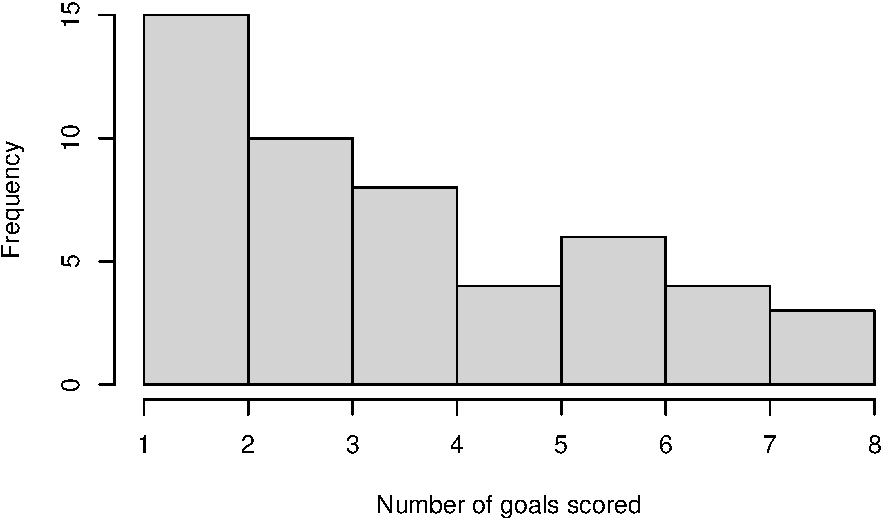
\includegraphics{_main_files/figure-latex/unnamed-chunk-16-1.pdf}

\begin{Shaded}
\begin{Highlighting}[]
\FunctionTok{mean}\NormalTok{(y)}
\end{Highlighting}
\end{Shaded}

\begin{verbatim}
## [1] 3.92
\end{verbatim}

We can model the number of goals scored using a Poisson distribution
\[
y \sim \hbox{Po}(\lambda).
\]
By Bayes' theorem, the posterior distribution is given by
\[
\pi(\lambda \mid \boldsymbol{y}) \propto \pi(\boldsymbol{y} \mid \lambda)\pi(\lambda). 
\]
The likelihood function is given by
\begin{align*}
\pi(\boldsymbol{y} \mid \lambda) &= \prod_{i=1}^50 \frac{e^{-\lambda}\lambda^{y_i}}{y_i!}\\
&= \frac{e^{-50\lambda}\lambda^{\sum y_i}}{\prod_{i=1}^50 y_i!} 
\end{align*}

R has a set of inbuilt functions for working with the Poisson distribution so we can rely on those to write functions for the likelihood and loglikelihood.

\begin{Shaded}
\begin{Highlighting}[]
\NormalTok{lambda }\OtherTok{\textless{}{-}} \FunctionTok{seq}\NormalTok{(}\DecValTok{0}\NormalTok{, }\DecValTok{10}\NormalTok{, }\FloatTok{0.01}\NormalTok{) }\CommentTok{\#grid of lambda values}
\NormalTok{likelihood.function }\OtherTok{\textless{}{-}} \ControlFlowTok{function}\NormalTok{(lambda, y) }\FunctionTok{prod}\NormalTok{(}\FunctionTok{dpois}\NormalTok{(y, lambda)) }\CommentTok{\#compute likelihood}
\NormalTok{log.likelihood.function  }\OtherTok{\textless{}{-}} \ControlFlowTok{function}\NormalTok{(lambda, y) }\FunctionTok{sum}\NormalTok{(}\FunctionTok{dpois}\NormalTok{(y, lambda, }\AttributeTok{log =} \ConstantTok{TRUE}\NormalTok{)) }\CommentTok{\#compute loglikelihood}
\NormalTok{likelihood }\OtherTok{\textless{}{-}} \FunctionTok{sapply}\NormalTok{(lambda,  likelihood.function, y) }\CommentTok{\#evaluate at grid of points}
\NormalTok{log.likelihood }\OtherTok{\textless{}{-}} \FunctionTok{sapply}\NormalTok{(lambda,  log.likelihood.function, y) }\CommentTok{\#evaluate at grid of points}

\CommentTok{\#Plot likelihood}
\FunctionTok{plot}\NormalTok{(lambda, likelihood, }
     \AttributeTok{xlab =} \FunctionTok{expression}\NormalTok{(mu), }\AttributeTok{ylab =} \StringTok{"likelihood"}\NormalTok{, }\AttributeTok{type =} \StringTok{\textquotesingle{}l\textquotesingle{}}\NormalTok{)}
\end{Highlighting}
\end{Shaded}

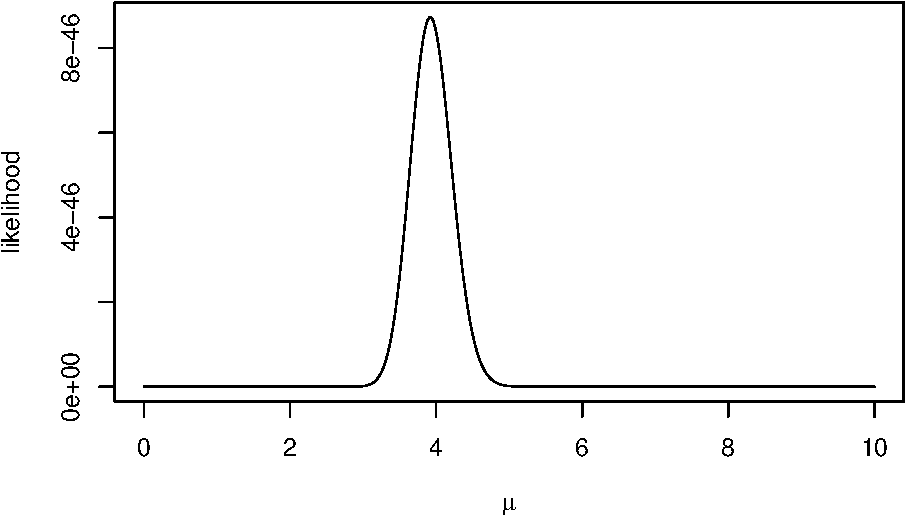
\includegraphics{_main_files/figure-latex/unnamed-chunk-17-1.pdf}

\begin{Shaded}
\begin{Highlighting}[]
\FunctionTok{plot}\NormalTok{(lambda, log.likelihood, }
     \AttributeTok{xlab =} \FunctionTok{expression}\NormalTok{(mu), }\AttributeTok{ylab =} \StringTok{"loglikelihood"}\NormalTok{, }\AttributeTok{type =} \StringTok{\textquotesingle{}l\textquotesingle{}}\NormalTok{)}
\end{Highlighting}
\end{Shaded}

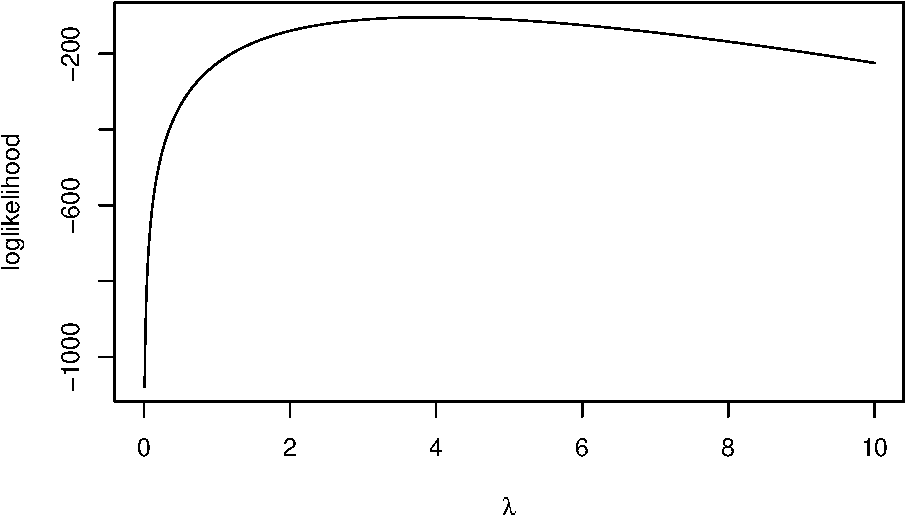
\includegraphics{_main_files/figure-latex/unnamed-chunk-17-2.pdf}
When coding posterior distributions, we often work on the log scale because the numbers can be smaller that R can deal with. The denominator with the factorial can get very large very quickly.

After speaking to football experts, we decide to place a normal prior distribution on \(\lambda\) with mean 5 goals and standard deviation one goal, i.e.
\[
\lambda \sim N(5, 1).
\]
The prior distribution can be plotted by

\begin{Shaded}
\begin{Highlighting}[]
\NormalTok{lambda   }\OtherTok{\textless{}{-}} \FunctionTok{seq}\NormalTok{(}\DecValTok{0}\NormalTok{, }\DecValTok{10}\NormalTok{, }\FloatTok{0.01}\NormalTok{) }\CommentTok{\#grid of lambda values}
\NormalTok{prior    }\OtherTok{\textless{}{-}} \FunctionTok{dnorm}\NormalTok{(lambda, }\DecValTok{5}\NormalTok{, }\DecValTok{1}\NormalTok{)}
\NormalTok{log.prior }\OtherTok{\textless{}{-}} \FunctionTok{dnorm}\NormalTok{(lambda, }\DecValTok{5}\NormalTok{, }\DecValTok{1}\NormalTok{, }\AttributeTok{log =} \ConstantTok{TRUE}\NormalTok{)}
\FunctionTok{plot}\NormalTok{(lambda, prior, }\AttributeTok{type =} \StringTok{\textquotesingle{}l\textquotesingle{}}\NormalTok{, }\AttributeTok{xlab =} \FunctionTok{expression}\NormalTok{(lambda), }\AttributeTok{ylab =} \StringTok{"density"}\NormalTok{)}
\end{Highlighting}
\end{Shaded}

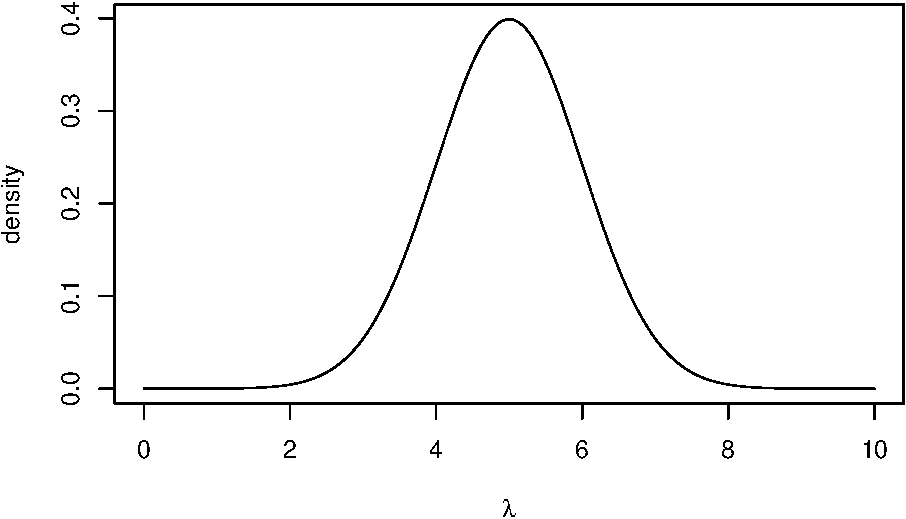
\includegraphics{_main_files/figure-latex/unnamed-chunk-18-1.pdf}

\begin{Shaded}
\begin{Highlighting}[]
\FunctionTok{plot}\NormalTok{(lambda, log.prior, }\AttributeTok{type =} \StringTok{\textquotesingle{}l\textquotesingle{}}\NormalTok{, }
     \AttributeTok{xlab =} \FunctionTok{expression}\NormalTok{(lambda), }\AttributeTok{ylab =} \StringTok{"log density"}\NormalTok{)}
\end{Highlighting}
\end{Shaded}

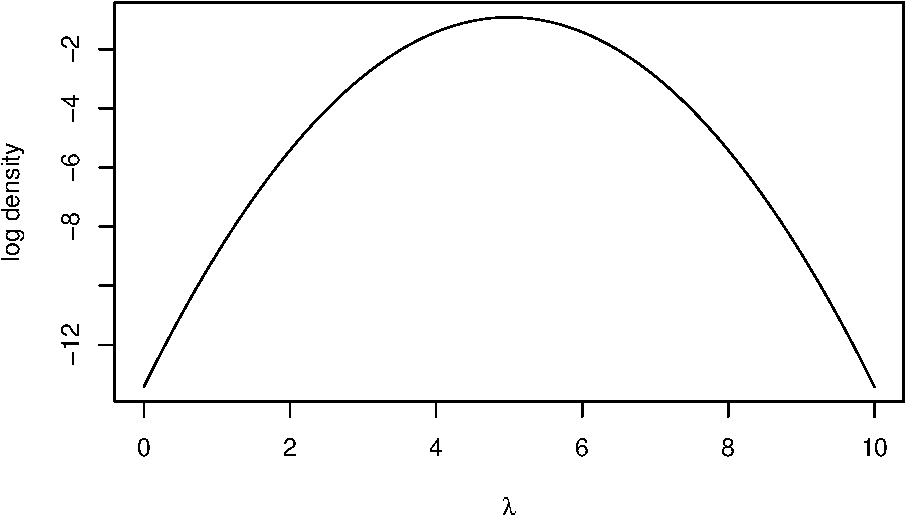
\includegraphics{_main_files/figure-latex/unnamed-chunk-18-2.pdf}

Writing the posterior distribution up to proportionality, we get
\[
\pi(\lambda \mid \boldsymbol{y}) \propto \exp\left(-50\lambda -\frac{1}{2}(\lambda - 5)^2\right)\lambda^{\sum y_i}.
\]
There is no closed form for this distribution and it is not that nice to work with. But with R, we can easily evaluate the posterior distribution at a grid of points.

\begin{Shaded}
\begin{Highlighting}[]
\NormalTok{posterior }\OtherTok{\textless{}{-}}\NormalTok{ prior}\SpecialCharTok{*}\NormalTok{likelihood}
\NormalTok{posterior }\OtherTok{\textless{}{-}}\NormalTok{ posterior}\SpecialCharTok{/}\FunctionTok{sum}\NormalTok{(posterior) }\CommentTok{\#normalise}
\FunctionTok{plot}\NormalTok{(lambda, posterior, }\AttributeTok{type =} \StringTok{\textquotesingle{}l\textquotesingle{}}\NormalTok{, }\AttributeTok{xlab =} \FunctionTok{expression}\NormalTok{(lambda), }
     \AttributeTok{ylab =} \StringTok{"posterior density"}\NormalTok{)}
\end{Highlighting}
\end{Shaded}

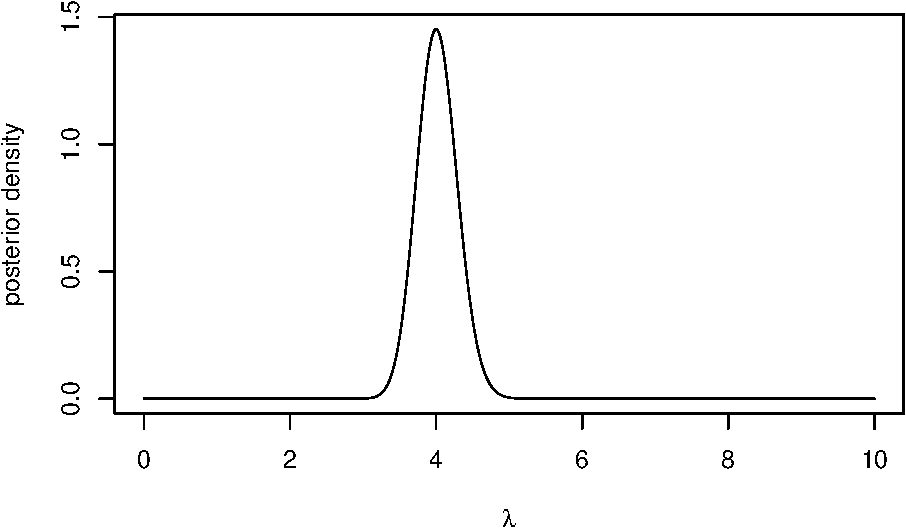
\includegraphics{_main_files/figure-latex/unnamed-chunk-19-1.pdf}

We can now visually inspect the posterior distribution and see that it has a strong peak around 4. One important statistic is the \textbf{maximum a posteriori estimation} or MAP estimate, this is the mode of the posterior distribution and it is a similar principle to the maximum likelihood estimate.

We can compute this using the command

\begin{Shaded}
\begin{Highlighting}[]
\NormalTok{lambda[}\FunctionTok{which.max}\NormalTok{(posterior)]}
\end{Highlighting}
\end{Shaded}

\begin{verbatim}
## [1] 4
\end{verbatim}

which shows the MAP estimate is exactly 4.
\end{example}

\begin{exercise}
Adapt the code in the Example above to use an exponential prior distribution with rate 0.1. Then derive the posterior distribution analytically and compare to the numerical version.
\end{exercise}

\begin{exercise}

You are given the data are exponentially distributed with rate \(\lambda,\) i.e.~\(Y_1, \ldots, Y_N \sim \hbox{Exp}(\lambda)\). Your prior belief is that \(\lambda \in (0, 1)\). Show that the posterior distribution \(\pi(\lambda \mid \boldsymbol{y})\) has no closed form when the prior distribution for \(\lambda \sim \hbox{Beta}(\alpha, \beta)\).

The data is given by

\begin{Shaded}
\begin{Highlighting}[]
\NormalTok{y }\OtherTok{\textless{}{-}} \FunctionTok{c}\NormalTok{(}\FloatTok{1.95}\NormalTok{, }\FloatTok{1.46}\NormalTok{, }\FloatTok{4.81}\NormalTok{, }\FloatTok{1.52}\NormalTok{, }\FloatTok{4.24}\NormalTok{, }\FloatTok{3.00}\NormalTok{, }\FloatTok{0.46}\NormalTok{, }\FloatTok{2.27}\NormalTok{, }\FloatTok{1.76}\NormalTok{, }\FloatTok{0.41}\NormalTok{)}
\end{Highlighting}
\end{Shaded}

\end{exercise}

By writing an R function to evaluate the likelihood function, evaute the posterior distribution for \(\lambda\) over a grid of points.

  \bibliography{book.bib,packages.bib}

\end{document}
